% §5 The affine landscape --- blueprint chapter 5 (blueprint/src/parts/05-*.tex). Written from the
% draft's §5 (Q-0288, 2026-10-04) on the template of sections 2 and 3 (spatial-hemigroup-affine #43).
% Every statement is transcribed verbatim from its node under a `% shared with blueprint` marker,
% with the paper statement's \label equal to the blueprint label (records/affine/
% transcribe-shared-statements.py), so that `linkage check` reports it `verbatim`. The drafting gate
% is records/affine/GATE-section-5.md.
%
% Files. The section is long, so it is split into parts: this file (the opening, 5.1 and 5.2),
% 05-table.tex (5.3, the overview table and the statement of thm:wedge-axis), 05-wedges.tex (5.4),
% 05-orbits.tex (5.5, 5.6), 05-smaller-groups.tex (5.7), 05-wedge-axis.tex (5.8, the proof of
% thm:wedge-axis) and 05-shape-adapted.tex (5.9, with the section's relation remark).
%
% Order (Q-0290, after the blind review records/affine/REVIEW-paper-section-5.md). The blueprint's,
% which follows the plan (notes/PLAN-article-structure.md, "§5"), with two changes: the overview
% table and the statement of thm:wedge-axis come right after 5.2, as the section's destination, with
% forward references (flag S4), the proof staying after every node it reads (5.8); and
% prop:stable-order-generated sits in 5.6 after prop:stable-exponent-cone, whose cone it reads (flag
% S12). 5.2 names the orbit sets of the smaller groups, proved in 5.7.
%
% Figure (Q-0290, review flag V1): fig-shape-plane.png in 5.2, from records/affine/fig-shape-plane.py
% with its output saved (fig-shape-plane-output.txt); no statement uses it.
%
% Appendices (Q-0290, the author's decision of 2026-10-04 to shorten by moving material, never
% deleting a statement): appendix-orders.tex (A), appendix-matern-cross-shape.tex (B),
% appendix-linear-flow.tex (C), appendix-similarity-loewner.tex (D), appendix-proofs.tex (E). A
% statement moved there goes whole, with its marker; the main text keeps a sentence naming it. A
% proof moved there leaves its statement here, followed by a pointer.
%
% Proofs. The proofs of record are the blueprint's. Short ones are transcribed; long ones are
% shortened to their decisive steps and headed "Sketch", which section 1.1 explains (the full proofs
% are in the deposited blueprint sources). Each proof cites the statements its node uses. The cited
% facts of section 2.6 an [A] node rests on are named, by number and \ref, before the node or, where
% a subsection has several such nodes on the same fact, once at the subsection's start (5.6, 5.7).
%
% Section 4 is written in parallel (Q-0287); its labels (def:gw-cascade-family,
% def:affine-cascade-family, eq:affine-gaussian, lem:operators-to-kernels, lem:affine-gauge,
% lem:parameter-space, thm:cascade-infinitely-divisible, lem:charfn-one-on-subspace,
% lem:single-ratio-cauchy, thm:rank-deficient-step, eq:one-step, thm:affine-rigidity) resolve once
% both sections are merged. Sections 5.1 and 5.8 take their reading of shape-adapted smoothing from
% lindeberg1994shape and lindeberg1997shape, read at the page (records/affine/READING-*.md; the
% stored copy of the 1997 article is the authors' report version, so it is cited by section only).
% The hub's experiments with a stable replacement are not used (the author, 2026-10-04).

\section{The affine landscape}\label{sec:landscape}

Theorem~\ref{thm:affine-rigidity} closes the classical corner of the axiom scheme: for $d \ge 2$, a
family covariant under the whole general linear group that cascades along every step of the Loewner order is an affine
Gaussian scale space. A user who wants another kernel at elliptical apertures, the Poisson kernel or a
\Matern{} kernel, has to give something up, and there are two things to give up. One is covariance, a
smaller group of linear maps of the image. The other is the cascade, an order smaller than the Loewner
order: fewer pairs of apertures $\Sigma, \Sigma'$ along which the record at $\Sigma'$ is a further
smoothing of the record at $\Sigma$. This section maps the families for each choice of the two
(Table~\ref{tab:landscape}). Every order used here is invariant under all of $\GL(d)$, so it pairs
with every group. Along the general linear row the families run from the affine orbits of all
rotation-invariant self-decomposable laws, each a round kernel stretched to every elliptical aperture,
on the rays (Proposition~\ref{prop:ray-families}), to the Gaussian alone, on the Loewner order. In
between, the orbit of the isotropic $\gamma$-stable law, $0 < \gamma < 2$, is a family along the
stable order of index $\alpha$ exactly when $\gamma \ge \alpha$ (Theorem~\ref{thm:wedge-axis}(3)), and
a \Matern{} orbit cascades along the rays and along no other step
(Proposition~\ref{prop:matern-steps}). What turns on the order is how fast an adapted aperture may
change its shape between two scales while the record stays a further smoothing
(\S\ref{sec:landscape-uses}). A smaller group admits more families in every column.

\S\ref{sec:landscape-uses} says what an affine scale space is used for, and what each
use asks of the axioms. \S\ref{sec:scale-shape} lists the groups and reads the Loewner order in volume
and shape. \S\ref{sec:landscape-table} gives the destination first: the overview table of the
families of each group along each order, with forward references. The rest fills it in. \S\ref{sec:invariant-wedges}
describes the invariant orders on positive definite matrices through their cones, which index the
chain of orders along which the general linear row is read. \S\ref{sec:affine-orbits} treats the base of the general linear row, the rays, and
\S\ref{sec:affine-stable-cone} the steps each orbit survives beyond them, up to the stable order on
$\PSD(d)$. \S\ref{sec:wedge-axis-proof} states and proves the theorem on the general linear row.
\S\ref{sec:shape-adapted} reads the practice of shape-adapted smoothing against the families, and
\S\ref{sec:smaller-groups} summarizes the rows of the smaller groups.
Appendices~\ref{app:classical}--\ref{app:wedge-axis} hold the proofs that \S\ref{sec:classical} and
this section defer, Appendix~\ref{app:wedge-axis} the complete proof of the theorem on the general
linear row. Appendices~\ref{app:orientation}--\ref{app:similarity} hold further results that the table
cites.

\subsection{What an affine scale space is for}\label{sec:landscape-uses}

The use of an affine scale space considered here is shape adaptation. An aperture whose shape
fits the local image structure measures the same thing in every affine image of a pattern. The
standard form of this is the iteration of Lindeberg and G\aa{}rding \sscite{lindeberg1994shape}. An
uncommitted, rotationally symmetric first stage, of variance $w$, fixes a point and an integration
scale.
The second-moment matrix of the image at that point then fixes the shape of the next aperture. The
image is smoothed again with the new covariance, and the step is repeated until the shape no longer
changes (\sscite{lindeberg1994shape}, p.~396, steps 1--4; \sscite{lindeberg1997shape}, \S6.2). The
iteration is the basis of the affine-invariant features of wide-baseline matching. Baumberg runs a
simplified form of it in the warped image with circular kernels at a fixed local scale, and scales
the warp to determinant $1$ (\sscite{baumberg2000reliable}, \S4.2, pp.~777--778). Mikolajczyk and
Schmid run it in the warped image too, normalizing the warp so that the patch is enlarged and never
shrunk (\sscite{mikolajczyk2004scale}, \S3.3, p.~72).
% Q-0314: Baumberg read at the page (READING-baumberg2000reliable.md); the TODO(source) is closed.
Each round convolves the original image. The affine scale-space representation is defined by one
convolution of the image for each covariance matrix (\sscite{lindeberg1994shape}, eq.~(15), p.~394),
and every round evaluates it at the new covariance. The second of the four steps divides the shape
matrix of the round by its least eigenvalue, so the local scale matrix, $w$ times that normalized
shape, keeps its least eigenvalue at $w$. The least amount of smoothing, and with it the suppression of noise, stays that of
the first stage (\sscite{lindeberg1997shape}, \S\S6.1--6.2).

Four uses can be read off this practice, and each asks something different of the axioms.
\begin{enumerate}
\item \emph{Shape selection.} At a point, choose the shape of the aperture that fits the local
structure. The selected shape must transform with the image, which needs the covariance group.
Lindeberg and G\aa{}rding select at fixed least smoothing. Selection at fixed volume, with
$\det\Sigma$ held constant, is the other natural normalization, and they reject it because it
overestimates the anisotropy (\sscite{lindeberg1997shape}, \S6.1). Baumberg's warp of determinant $1$
is this normalization. At fixed volume no Loewner step leads from the isotropic first stage to another
shape: if $\Sigma \le \Sigma'$ and $\det\Sigma = \det\Sigma'$, the relative step
$\Sigma^{-1/2}\Sigma'\Sigma^{-1/2}$ has eigenvalues at least $1$ with product $1$, so
$\Sigma' = \Sigma$. Under that normalization even the Gaussian reaches an adapted aperture only by
measuring the image afresh.
\item \emph{Following a shape across scale.} Between stages the adapted aperture grows. Along a ray
$\Sigma \to \lambda^2\Sigma$ the coarser record is a further smoothing of the finer one only if the
rays belong to the order.
\item \emph{Changing shape.} When the shape is re-estimated as the scale grows, the adapted apertures trace
a curve in scale and shape, not a ray. The curve is a cascade only if each of its steps lies in the
order, and each family limits how fast the shape may change along it.
\item \emph{Singularity theory over the larger group.} A larger covariance group gives more to take
the quotient by, and a larger parameter space $(x, \Sigma)$ in which to study the deep structure of
the image. This use is not treated here (\S\ref{sec:conclusion}).
\end{enumerate}

So the question splits into a choice of group and a choice of order.
% Round 3 (content review), C-R6 and E-R7: shape selection in the sense used here.
Shape selection, in the sense used here, transports a shape with the image under every linear map, so
it needs a group that carries every shape to every other, as $\GL(d)$ does on $\PD(d)$. Among the families covariant under $\GL(d)$, what differs is the order. A family cascades
along a step $\Sigma \to \Sigma'$ when its kernel at $\Sigma'$ is its kernel at $\Sigma$ convolved with
a probability measure, the \emph{increment}. The coarser record is then a further smoothing of the
finer one. That the increment is a probability measure carries weight
(Remark~\ref{rem:positivity}).
% Round 3 (content review), C-R5 and A.R4: the name for a change with no probability increment.
Off the order the axioms ask for no increment. A change of aperture with no increment that is a
probability measure is called a \emph{re-measurement} of the original image. The coarser record is then
not a further smoothing of the finer one.
\S\ref{sec:shape-adapted} returns to the four uses with the results in hand.

\subsection{The groups, and the Loewner order in volume and shape}\label{sec:scale-shape}

The landscape has two axes, and this subsection sets out both. Its rows are groups, and the list below
says which shapes each group carries to which. Its columns are the rays, the stable orders and the
Loewner order. Each contains the rays and is contained in the Loewner order
(Proposition~\ref{prop:similarity-stable-order-families}(1) for the stable orders), so every step of
every column is a Loewner step. Read in coordinates of volume and shape, the Loewner order says two
things a user of shape adaptation needs (Lemma~\ref{lem:loewner-scale-shape}). Two distinct apertures
of the same volume are never ordered, so a change of shape at fixed volume is never a further
smoothing, for the Gaussian either. And one step can change the shape only within a limit set by the
growth of the volume. Figure~\ref{fig:shape-plane} draws that limit in the plane.

A group of the scheme is a closed subgroup of $\GL(d)$ that contains the dilations, acting on
$\PSD(d)$ by $A \cdot \Sigma = A\Sigma A^{\tp}$ (Definition~\ref{def:gw-cascade-family}). The
landscape uses these groups:
\begin{itemize}
\item $\GL(d)$ and its orientation-preserving subgroup $\GL^+(d)$, which act transitively on
$\PD(d)$, with stabilizers of $I$ the orthogonal group $\Orth(d)$ and the rotation group
$\mathrm{SO}(d)$;
\item the similarities $\mathrm S(d) = \{cQ : c > 0,\ Q \in \Orth(d)\}$, whose orbits in
$\PSD(d) \setminus \{0\}$ are indexed by the normalized spectrum
(Proposition~\ref{prop:similarity-ray-families}(1));
\item the diagonal matrices with positive entries, $\mathrm D_+(d)$, whose orbits in $\PD(d)$ are
indexed by the correlation matrices (Proposition~\ref{prop:diagonal-ray-families}(1));
\item the dilations $\{\lambda I : \lambda > 0\}$, which each of them contains.
\end{itemize}
The special linear group and $\Orth(d)$ contain no dilations, so neither is the group of a wedge
datum. They enter as the shape part of $\GL(d)$ and as the stabilizer of $I$. A
\emph{one-parameter group} is the set $\{e^{sB} : s \in \RR\}$ of the linear maps generated by one real
$d \times d$ matrix $B$, with $e^{sB}$ the matrix exponential, so that $e^{sB}e^{s'B} = e^{(s+s')B}$.
For $B = I$ it is the group of dilations $e^s I$, for a skew-symmetric $B$ a group of rotations, and
for $B = \diag(1, 0, \dots, 0)$ the stretchings $\diag(e^s, 1, \dots, 1)$ of the first axis. Such a
group moves an aperture $\Sigma_0$ along the curve $e^{sB}\Sigma_0e^{sB^{\tp}}$, which is not an order
on $\PSD(d)$, and its families are treated on their own in Appendix~\ref{app:linear-flow}.

\paragraph{Orientation.} For $d \ge 2$ the orientation-preserving group gives no row of its own. An
order invariant under $\GL^+(d)$ is invariant under $\GL(d)$, and the $(\GL^+(d), W)$-cascade families
of kernels and of operators are the $(\GL(d), W)$-cascade families
(Proposition~\ref{prop:glplus-families}, stated and proved in Appendix~\ref{app:orientation}). So for
$d \ge 2$ every statement made below for $(\GL(d), W)$ holds verbatim for $(\GL^+(d), W)$.

The space $\PD(d) = \GL(d)/\Orth(d)$ has natural coordinates of volume and shape, and the Loewner
order of Definition~\ref{def:affine-cascade-family} reads simply in them. The reading tells a vision
application which comparisons across scale and shape exist at all.

% shared with blueprint lem:loewner-scale-shape
\begin{lemma}[the Loewner order in scale--shape coordinates]\label{lem:loewner-scale-shape}
For $\Sigma \in \PD(d)$ put $t(\Sigma) := (\det\Sigma)^{1/2d}$, the \emph{volume scale}, and
$S(\Sigma) := t(\Sigma)^{-2}\Sigma$, the \emph{shape}, so that $\det S(\Sigma) = 1$. Let
$\Sigma_1, \Sigma_2 \in \PD(d)$, $t_k := t(\Sigma_k)$, $S_k := S(\Sigma_k)$, and let
$n_1 \le \dots \le n_d$ be the eigenvalues of the \emph{relative shape}
$N := S_1^{-1/2}S_2S_1^{-1/2}$, so that $n_1 \cdots n_d = 1$.
\begin{enumerate}
\item $\Sigma_1 \le \Sigma_2$ if and only if $n_1 \ge (t_1/t_2)^2$.
\item \emph{(No order within a scale.)} If $\Sigma_1 \le \Sigma_2$ then $t_1 \le t_2$, with
equality only if $\Sigma_1 = \Sigma_2$; and $\Sigma_1 \le \Sigma_2$ with $S_1 = S_2$ holds exactly
when $\Sigma_2 = \lambda^2\Sigma_1$ with $\lambda \ge 1$.
\item \emph{(A speed limit on shape.)} If $\Sigma_1 \le \Sigma_2$ then
$(t_1/t_2)^2 \le n_1 \le n_d \le (t_2/t_1)^{2(d-1)}$, so the anisotropy gained,
$\sqrt{n_d/n_1}$, is at most $(t_2/t_1)^d$. Conversely, for every $t_2 \ge t_1$ and every
$N \in \PD(d)$ with $\det N = 1$ and least eigenvalue at least $(t_1/t_2)^2$,
$\Sigma_2 := t_2^2\,S_1^{1/2}NS_1^{1/2}$ satisfies $\Sigma_1 \le \Sigma_2$, $t(\Sigma_2) = t_2$, and
has relative shape $N$.
\item \emph{(The plane.)} Let $d = 2$ and
$\delta(S_1,S_2) := \bigl((\log n_1)^2 + (\log n_2)^2\bigr)^{1/2}$. For $t_2 \ge t_1$, the shapes
$S(\Sigma_2)$ of the $\Sigma_2 \ge \Sigma_1$ with $t(\Sigma_2) = t_2$ are exactly the shapes $S$
with $\det S = 1$ and $\delta(S_1,S) \le 2\sqrt2\,\log(t_2/t_1)$.
\end{enumerate}
\end{lemma}

Clause (2) says that a selection of shape at fixed volume is a re-measurement for every family, the
Gaussian included. No two distinct apertures of the same volume are comparable, so no cascade axiom
bears on such a selection. Clause (3) is a speed limit on the anisotropy gained per step, and it is
the Gaussian's, since the Gaussian cascades along the whole Loewner order. The stable orders of
\S\ref{sec:affine-stable-cone} have narrower limits of the same form
(Proposition~\ref{prop:stable-step-cone}(3)). Figure~\ref{fig:shape-plane} draws both in the plane:
the shapes one step can reach form discs around the starting shape, nested by the order, and the
apertures of shape-adapted smoothing lie on the edge of the Loewner disc. The number
$\delta(S_1,S_2)$, the norm $(\tr(\log N)^2)^{1/2}$ of the logarithm of the relative shape, is the
distance between $S_1$ and $S_2$ in the affine-invariant Riemannian metric on the positive definite
matrices, the metric invariant under $\Sigma \mapsto A\Sigma A^{\tp}$ (\sscite{pennec2006riemannian},
\S\S3.2--3.3, pp.~46--47; \sscite{bhatia2007positive}, Thm.~6.1.6 and (6.13), p.~205).
% Q-0314: Bhatia ch. 6 and Pennec-Fillard-Ayache read at the page (READING-bhatia2007positive.md,
% READING-pennec2006riemannian.md); the TODO(source) is closed. Neither source states the
% hyperbolic-plane reading in the pages read, so it stays unproved and unused.
Clauses (1) and (2) rest on textbook facts about the Loewner order. For
$\Sigma_1, \Sigma_2 \in \PD(d)$, $\Sigma_1 \le \Sigma_2$ exactly when every eigenvalue of
$\Sigma_1^{-1/2}\Sigma_2\Sigma_1^{-1/2}$ is at least $1$ (\sscite{horn2012matrix}, Thm.~7.7.3(a),
p.~494). The eigenvalues and the determinant increase along the order (Cor.~7.7.4(c) and~(e),
p.~495).
The proof of the lemma, from the congruence $M = \Sigma_1^{-1/2}\Sigma_2\Sigma_1^{-1/2} =
(t_2/t_1)^2N$, is in Appendix~\ref{app:proofs}.

\begin{figure}[!tbp]
\centering
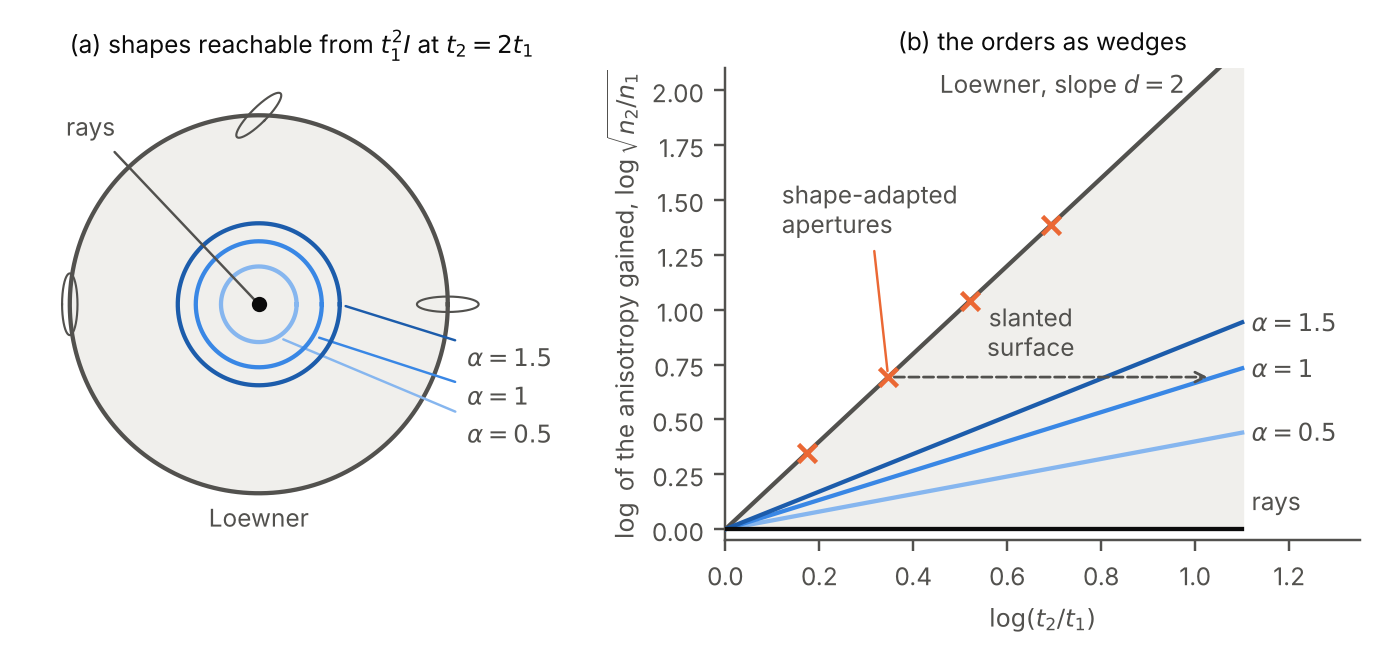
\includegraphics[width=\textwidth]{fig-shape-plane.png}
\caption{The plane, $d = 2$: one step from the isotropic aperture $\Sigma_1 = t_1^2I$. (a) The shapes
$S(\Sigma_2)$, $\det S = 1$, reachable at volume scale $t_2 = 2t_1$, in a chart whose radius is the
distance $\delta(I, S)$ of Lemma~\ref{lem:loewner-scale-shape}(4) and whose angle is twice the
orientation of the major axis.
% Round 2 (presentation review), item 10 (VERIFY-round2-structure-paper.md § 10.4): why the angle is
% doubled (det S = 1, so log S is trace-free), and the dashed arrow of panel (b), checked against
% section 4.8 and records/affine/fig-shape-plane-output.txt (y = log 2, x from 0.3466 to 1.0397).
Rotating the aperture through $\theta$ turns $\log S$, a point of the plane of trace-free symmetric
matrices, through $2\theta$, so orthogonal orientations lie at opposite points. The Loewner order reaches the disc of radius $2\sqrt2\log(t_2/t_1)$
(Lemma~\ref{lem:loewner-scale-shape}(4)); the stable order of index $\alpha$ the disc of radius
$2\sqrt2\,\frac{\alpha}{2+\alpha}\log(t_2/t_1)$ (Proposition~\ref{prop:stable-step-cone}(3)); the rays
only the centre. The ellipses are apertures on the Loewner edge in three orientations. (b) The same
orders in the logarithm of the anisotropy gained, $\sqrt{n_2/n_1}$, against the logarithm of the scale
ratio: slopes $d$, $d\alpha/(d+\alpha)$ and $0$. The crosses are the apertures of shape-adapted smoothing
at anisotropy $n_2/n_1 = 2$, $4$, $8$, $16$, reached from the
isotropic first stage (Proposition~\ref{prop:shape-adapted-apertures}), which lie on the Loewner edge.
The dashed arrow is the step for the surface at slant $60^\circ$ of \S\ref{sec:shape-adapted}, at
log-anisotropy $\log 2$. It runs from the aperture of shape-adapted smoothing on the Loewner edge to the edge of the stable order of
index $\alpha = 1$, which reaches that shape only at twice the volume scale. Computed, with the
discs checked against the two orders on random steps, by a script deposited with the paper.}
\label{fig:shape-plane}
\end{figure}

% §5.3 The landscape at a glance --- blueprint chapter 5, part 05-table.tex (Q-0288; moved forward
% to right after 5.2 in Q-0290, review flag S4: the table, with forward references, and the statement
% of thm:wedge-axis are the section's destination; the theorem's proof is 5.8, 05-wedge-axis.tex,
% after every node it reads). Included from 05-landscape.tex; the conventions are in that file's
% header. The table is built from the nodes, each cell citing the statements it summarizes; every
% cell was compared with its statements for lost hypotheses (WRITING.md § 5, "a summary drops
% hypotheses"). The table is for d >= 2, the dimension in which the general linear Loewner cell and
% the stable-order cells are stated. The one node is thm:wedge-axis; the remark on positivity is the
% plan's (notes/PLAN-article-structure.md, "§5"), as far as it is proved, and states no signed family
% (the author, 2026-10-04).
% Q-0309 (fix group 2, review flag 10): the formal statement of thm:wedge-axis moved to 5.8
% (05-wedge-axis.tex), where its vocabulary exists, before its proof; this subsection keeps the table
% and an informal statement of the theorem (the paragraph "The general linear row along the chain").

\subsection{The landscape at a glance}\label{sec:landscape-table}

Table~\ref{tab:landscape} answers, for each choice of covariance group and of the pairs of apertures
along which the record must be a further smoothing, which kernels are available. It has the groups of \S\ref{sec:scale-shape}
as rows and three orders as columns, for $d \ge 2$, and every cell has an entry, citing the statements
it summarizes in \S\S\ref{sec:invariant-wedges}--\ref{sec:smaller-groups} or in the appendices. The
cells use these terms.
\begin{itemize}
\item The \emph{ray order} relates $\Sigma$ to its multiples $c\,\Sigma$, $c \ge 1$, and $0$ to
everything.
\item The \emph{stable order} $\le_\alpha$, $0 < \alpha < 2$, relates two definite matrices when the
relative step $M = \Sigma^{-1/2}\Sigma'\Sigma^{-1/2}$ has $\lambda_{\min}(M)^{d+\alpha} \ge \det M$, and
adds the origin and the rays (Proposition~\ref{prop:similarity-stable-order-families}(1)). It lies
between the rays and the Loewner order.
% Round 3 (content review), C section 7 (VERIFY-round3-landscape-orbits-paper.md item 30): the pointer
% for "step set", which this page uses before Proposition 4.2.
It is the order of the step set (Proposition~\ref{prop:invariant-orders}, \S\ref{sec:affine-stable-cone})
of the stable orbit of index $\alpha$, the linear images $(\Sigma^{1/2})_*S_\alpha(I)$ of the isotropic $\alpha$-stable law, whose
transform is $e^{-|\omega|^\alpha}$ (Lemma~\ref{lem:elliptical-stable} and
Proposition~\ref{prop:stable-step-cone}). At $\alpha = 1$ that law is the kernel of the Poisson scale
space at unit scale (\S\ref{sec:classical-prior-art}). And it is the order generated by the cone of directions
$C_\alpha := \{X \in \PSD(d) : (d+\alpha)\,\lambda_{\min}(X) \ge \tr X\}$
(Proposition~\ref{prop:stable-order-generated}); $C_0$ gives the rays and $C_\infty := \PSD(d)$ the
Loewner order.
\item The \emph{frame} is the coordinate frame, the axes of the sampling grid along which the
positive diagonal group $\mathrm D_+(d)$ rescales. The \emph{frame's shapes} are the positive definite
diagonal matrices, the apertures whose axes are those of the frame, and they are the orbit of $I$
under $\mathrm D_+(d)$.
% Round 2 (presentation review), item 4 (VERIFY-round2-structure-paper.md § 4.1): D_s and
% Delta(Sigma), defined as in Propositions F.2 and F.4; Corr(d) is not printed in the table.
For $s \in (0,\infty)^d$ write $D_s := \diag(s_1,\dots,s_d)$, so that the frame's shapes are the
$D_s^2$, and write $\Delta(\Sigma) := \diag(\Sigma_{11},\dots,\Sigma_{dd})$ for the diagonal of $\Sigma$.
% Round 2 (presentation review), item 4: the term B-self-decomposable and sym B, as in
% Proposition 4.10.
\item The \emph{exponent cone} $\mathfrak k_\alpha$ of the stable law is the set of matrices $B$ for which
$S_\alpha(I)$ is its own image under $e^{-tB}$ convolved with a residual, for every $t > 0$. A law with
this property is \emph{$B$-self-decomposable}, or operator-self-decomposable with exponent $B$
(Proposition~\ref{prop:stable-exponent-cone}). The symmetric part of $B$ is
$\mathrm{sym}\,B := \tfrac12(B + B^{\tp})$.
\item \emph{Anisotropy} is measured by the exponent spread $\operatorname{es}$ of the non-Gaussian part,
the least $K \ge 1$ with $\psi(Q\omega) \le K\,\psi(\omega)$ for every $Q \in \Orth(d)$. It is set
against the eccentricity $\operatorname{ecc}(\Sigma)$ of the aperture, the ratio of its extreme
eigenvalues. Both are defined again where they are used, in Proposition~\ref{prop:similarity-stable-order-kernels}.
\item A non-Gaussian part is \emph{shape-blind} when it is rotation invariant at every $\Sigma$, so that
it sees the size of the aperture and not its shape. It is shape-blind \emph{at the origin} when its
\Levy{} measure has the same rate near the origin in every direction.
\item The profile entries concern a rotation-invariant law with no Gaussian part whose \Levy{}
density at $x$ is $k(|x|)\,|x|^{-d}$, with $k$ nonincreasing, its \emph{profile}, and the law is
written $\nu_k$. They use the
dilation ratio $R(\lambda) := \inf\{k(r/\lambda)/k(r) : r > 0,\ k(r) > 0\}$, $\lambda \ge 1$, and the
lower exponent $\beta_-(k) := \inf_{\lambda > 1}\log R(\lambda)/\log\lambda$
(Proposition~\ref{prop:orbit-step-cone} and Lemma~\ref{lem:dilation-ratio}).
% Round 2 (presentation review), item 4 (§ 4.2): the gloss of R(lambda) >= lambda^alpha. With
% s = r/lambda it reads k(s) s^alpha >= k(r) r^alpha for s <= r.
The condition $R(\lambda) \ge \lambda^\alpha$ for every $\lambda \ge 1$ says that $r^\alpha k(r)$ is
nonincreasing: towards the origin the profile grows at least like $r^{-\alpha}$.
\end{itemize}
The one-parameter row lies outside the scheme, a curve not being an order on $\PSD(d)$, and is listed
below the others.

\begin{table}[tp]
\centering
\small
\setlength{\tabcolsep}{4pt}
\renewcommand{\arraystretch}{1.15}
\begin{tabular}{@{}p{0.12\textwidth}p{0.27\textwidth}p{0.28\textwidth}p{0.27\textwidth}@{}}
\toprule
$G$ & rays & stable order $\le_\alpha$, $0 < \alpha < 2$ & Loewner order \\
\midrule
$\GL(d)$ &
the orbits $(\Sigma^{1/2})_*\mu_I$ of the rotation-invariant self-decomposable laws $\mu_I \ne \delta_0$,
one family for each law (Propositions~\ref{prop:ray-families} and~\ref{prop:gw-ray-families}(3)) &
% Round 3 (content review), E i and C-R3 (the author's decision D10): the cell is complete,
% Proposition 4.22(2) with C5.
the orbits of exactly the laws $N(0, aI)$, $a > 0$, and $N(0, aI) * \nu_k$, $a \ge 0$, with $k$
right-continuous and $\beta_-(k) \ge \alpha$; among the stable orbits, exactly those of index $\gamma \ge \alpha$
(Theorem~\ref{thm:wedge-axis}(3), Proposition~\ref{prop:wedge-axis-profiles},
Lemma~\ref{lem:dilation-ratio}(3)) &
the affine Gaussian scale spaces only (Theorem~\ref{thm:affine-rigidity}) \\
\addlinespace
similarities $\mathrm S(d)$ &
continuous covariant fields of symmetric self-decomposable laws over the shapes, with orbits indexed by
the normalized spectrum; the isotropic members are the rotation-invariant self-decomposable laws
$\ne \delta_0$, and none fixes its family (Proposition~\ref{prop:similarity-ray-families}) &
every family's kernels are symmetric infinitely divisible with
$\operatorname{es}(\psi_\Sigma) \le 4\operatorname{ecc}(\Sigma)^{(d+\alpha)/\alpha}$; contains the restrictions of
the $\GL(d)$ cell and of the Loewner cell, and a family in neither
(Proposition~\ref{prop:similarity-stable-order-kernels}) &
% Round 3 (content review), A.R9: F.3(4) and its witness F.3(3)(ii).
the isotropic members of the ray cell, each with a shape-blind family
(Proposition~\ref{prop:similarity-ray-families}(3)--(4)); every family's kernels are infinitely divisible with
$\operatorname{es}(\psi_\Sigma) \le 4\operatorname{ecc}(\Sigma)$
(Proposition~\ref{prop:similarity-stable-order-kernels}(2)); a uniform bound when the \Levy{} measures
at the thinnest apertures stay comparable to the isotropic member's, and none in general
(Propositions~\ref{prop:similarity-general-bounded-shape}, \ref{prop:similarity-cascade-families}
and~\ref{prop:similarity-degenerate-family}); for a profile bounded at the origin, shape-blind at the
origin (Proposition~\ref{prop:similarity-general-index-zero}) and need not be beyond it
% Round 2 (presentation review), item 4 (§ 4.3): "not beyond it" narrowed to "need not be beyond
% it"; one example family backs it, and the shape-blind families of the cell are rotation invariant.
(Proposition~\ref{prop:similarity-line-family}(3)); not every family is a Gaussian convolved with a
shape-blind part (Proposition~\ref{prop:similarity-stable-family}(3)) \\
\addlinespace
positive diagonal $\mathrm D_+(d)$ &
on the frame's shapes the images $(D_s)_*\mu_I$ of any self-decomposable $\mu_I \ne \delta_0$, not
necessarily products; orbits in $\PD(d)$ indexed by the correlation matrices; a rotation-invariant member fixes
no family off the frame's shapes (Proposition~\ref{prop:diagonal-ray-families}) &
on the frame's shapes $(D_s)_*\mu_I$ with $\mu_I$ operator-self-decomposable for every diagonal exponent
in $\mathfrak k_\alpha$, a necessary condition, and whether every such law is the isotropic member of a
family is open; strictly between the restricted Loewner cell and the ray cell, and not the union of the
restrictions of the Loewner and $\GL(d)$ cells; off the frame's shapes not described
(Proposition~\ref{prop:diagonal-stable-order-families}) &
on the frame's shapes the products $(s_1)_*\nu_1 \otimes \dots \otimes (s_d)_*\nu_d$ of self-decomposable
laws on the line (Propositions~\ref{prop:fixed-frame-families} and~\ref{prop:diagonal-ray-families}(3));
off the frame's shapes one extension, $(\Delta(\Sigma)^{1/2})_*(\nu_1 \otimes \dots \otimes \nu_d)$, the
families not described \\
\midrule
% Round 3 (content review), C-S6: what "with rotations" meant.
\multicolumn{4}{@{}p{0.98\textwidth}@{}}{\emph{One linear flow} $\{e^{sB}\}$, $B$ with a skew part allowed, along the
curve $e^{sB}\Sigma_0e^{sB^{\tp}}$: the families are the $B$-self-decomposable laws
(Proposition~\ref{prop:one-parameter-families}); for a contracting flow a rotation-invariant non-Gaussian
member exists exactly when $\tr B < (d+2)\lambda_{\min}(\mathrm{sym}\,B)$
(Proposition~\ref{prop:anisotropy-budget}).} \\
\bottomrule
\end{tabular}
\caption{The affine landscape for $d \ge 2$: the families of each group along each order. The four
corners of the scheme (Definition~\ref{def:gw-cascade-family}) are the cells of the first two rows in
the ray and the Loewner columns. Each cell cites the statements it summarizes. The cells of the general
linear group are complete, and \S\ref{sec:conclusion} says how far the others go.}
% Round 3 (content review), A.R1 and C-R2 (PLAN-review-response-paper.md R3.1, "taken unless vetoed"):
% the complete cells named in the caption, three since D10.
\label{tab:landscape}
\end{table}

\paragraph{The inclusions.} A family of a larger group or a larger order restricts to every smaller
datum, with the same kernels from scale zero (Lemma~\ref{lem:gw-kernels-from-origin}(1)), so in each column
the cells grow from the general linear row to each smaller group's row, and along each row towards the
rays. These inclusions are known to be strict:
\begin{itemize}
\item along the general linear row, at every step of the chain up to $\alpha = 2$
(Theorem~\ref{thm:wedge-axis}(3));
\item from the $\GL(d)$ cell and the restricted Loewner cell to the cell (similarities, stable order)
(Proposition~\ref{prop:similarity-stable-order-kernels}(3));
\item from the restricted Loewner cell to the stable cell, and from there to the ray cell, in the diagonal
row (Proposition~\ref{prop:diagonal-stable-order-families}(4)), and so from the restricted (diagonal,
Loewner) cell to the (diagonal, rays) cell (Proposition~\ref{prop:diagonal-ray-families}(4)).
\end{itemize}
% Round-1 external review (Gemini; PLAN-review-response-paper.md, D3): the paragraphs "The isotropic
% members" (moved to section 1, "Smaller groups") and "The general linear row along the chain" (said by
% section 1 and section 4.7) are folded into section 1.

% Q-0317 (the blind register review, second half flag 25): rem:positivity moved to section 3.4,
% beside the rigidity it is about.

% §5.4 Invariant wedges --- blueprint chapter 5, part 05-wedges.tex (Q-0288). Included from
% 05-landscape.tex; the conventions are in that file's header. The nodes are linear algebra; since
% Q-0281 wave 2, group F (the author's decision of 2026-10-05) lem:spectral-cones(2) cites C4 (ledger
% A9) in place of its compound-matrix proof, and the nodes that read it spend it. Q-0290: lem:spectral-cones, thm:cone-orders (whole, the node not
% being split; this file states its four clauses in words) and the proof of prop:invariant-orders are
% in appendix A; prop:stable-order-generated is in 5.6, after the exponent cone it reads (review flag
% S12). The prior-art paragraph cites the readings recorded in
% records/affine/READING-{lawson1989ordered,hilgert1989lie,hilgert1997causal,faraut1994analysis}.md,
% with the page anchors of the nodes' annotations; no proof depends on them. The chain of cones and
% the general linear row along it (thm:wedge-axis) are stated in 5.3.
% Q-0309 (fix group 2, review flag 35): thm:cone-orders is stated here, in place of the paraphrase of
% its four clauses, since its clause (4) defines the order thm:wedge-axis is stated on; its proof,
% lem:spectral-cones and the proof of prop:invariant-orders are in the proof appendix (app:proofs).

\subsection{Invariant wedges}\label{sec:invariant-wedges}

An order of the landscape says which changes of aperture must be further smoothings. This subsection
asks which orders there are, and how to describe one by what may happen in an instant. For the
Gaussian the answer is familiar. Its aperture may grow in any direction, $\Sigma(t)$ moving with a
positive semidefinite velocity $\Sigma'(t)$, and the pairs joined by such a curve are those of the
Loewner order (Proposition~\ref{prop:stable-order-generated}(1), at $\alpha = \infty$). The rays allow
only a velocity that is a nonnegative multiple of $\Sigma(t)$, a growth without a change of shape. An
order in between allows at each aperture a cone of velocities, the \emph{cone field}, and relates two
apertures when a curve whose velocity stays in the cones joins them. The main result,
Theorem~\ref{thm:cone-orders}, says that the closed invariant partial orders on $\PD(d)$ that arise
in this way are exactly those whose steps can be taken in fractions, and that every step of such an
order is reached along one curve, with no limit of curves needed. The rays, the stable orders and the
Loewner order are of this kind, the members $C_0$, $C_\alpha$ and $C_\infty$ of one chain of cones
(Proposition~\ref{prop:stable-order-generated}).

% Pass 6, the author's review of section 4.4 (2026-11-02; records/affine/REVIEW-author-paper-affine.md):
% "some, preferably geometric, intuition about what the cone and wedges are and how they will be
% used". Paper-only prose. The plane computation: X = [[a+u, v], [v, a-u]] has eigenvalues
% a +- r, r = sqrt(u^2+v^2); a rotation by phi rotates (u, v) by 2 phi and fixes a, a reflection
% reflects (u, v); so an O(2)-invariant closed convex cone with I in it and no line is
% {r <= k a}, k >= 0. PSD(2) is k = 1. C_alpha of prop:stable-order-generated, (2+alpha) lambda_min
% >= tr, is (2+alpha)(a-r) >= 2a, that is k = alpha/(alpha+2): C_0 has k = 0, C_2 has k = 1/2, and
% k -> 1 as alpha -> infinity. thm:wedge-axis(2) read in the plane: beta(C) = max tr X/lambda_min(X)
% - 2 = 2k/(1-k) for the round cone of opening k < 1, so (a) k > 1 (not in PSD(2)): no family;
% (b) k = 1 (a singular member): the Gaussian only; (c) k < 1: a non-Gaussian family exists iff
% beta < 2 iff k < 1/2.
\paragraph{A picture in the plane.} For $d = 2$ the cones can be drawn. Write a symmetric matrix as
$X = \bigl(\begin{smallmatrix} a+u & v \\ v & a-u \end{smallmatrix}\bigr)$, so that $\Sym(2)$ is a
space of three dimensions with coordinates $(a, u, v)$, and $X$ has the eigenvalues
$a \pm \sqrt{u^2+v^2}$. Read $X$ as the velocity of an aperture at $I$. Then $a$ is its growth in
size, $\sqrt{u^2+v^2}$ its rate of change of shape, and the angle of $(u, v)$ the direction in which
it stretches. A rotation of the plane by an angle $\phi$ rotates $(u, v)$ by $2\phi$ and leaves $a$
alone. So a closed convex cone that is invariant under rotations, contains $I$ and contains no line is
a round cone about the axis of the multiples of $I$,
\[
  \sqrt{u^2+v^2} \le k\,a \qquad \text{for some } k \ge 0 .
\]
Its opening $k$ bounds how fast the shape may change against how fast the aperture grows
(Figure~\ref{fig:cones-plane}). The rays
are the axis alone, $k = 0$. The Loewner order allows every positive semidefinite velocity, the cone
$k = 1$ of half-angle $45^\circ$, and a wider cone allows an aperture to shrink in some direction. The
cone $C_\alpha$ of the chain has $k = \alpha/(\alpha+2)$, so the stable orders, $0 < \alpha < 2$, are
the cones narrower than $k = \frac12$. The cone field carries the cone at $I$ to every aperture by the
group, and the order relates two apertures when a curve whose velocity stays in the cones joins them.
Lie theory calls a closed convex cone a \emph{wedge} (\S\ref{sec:affine-covariance}), and these
wedges, which contain no line, are the tangent objects through which it studies such orders. The rest
of the section uses them in two ways. Each affine orbit has its own set of steps along which it
cascades, and \S\S\ref{sec:affine-orbits}--\ref{sec:affine-stable-cone} find it for the orbits of
interest: the rays alone for the \Matern{} kernels, the order of $C_\gamma$ for the stable kernel of
index $\gamma$. And in the plane
Theorem~\ref{thm:wedge-axis} reads off the opening. A cone with $k < \frac12$ carries non-Gaussian
families, a cone with $\frac12 \le k \le 1$ carries only the affine Gaussian scale spaces, and a cone
with $k > 1$ carries none.

% Pass 6 (the author's request of 2026-11-02, "Add the figure please"): fig-cones-plane.png, drawn by
% records/affine/fig-cones-plane.py with its output saved (fig-cones-plane-output.txt); the script
% checks the openings k = alpha/(alpha+2), PSD(2) = {r <= a} and beta = 2k/(1-k) before drawing. No
% statement uses it.
\begin{figure}[t]
\centering
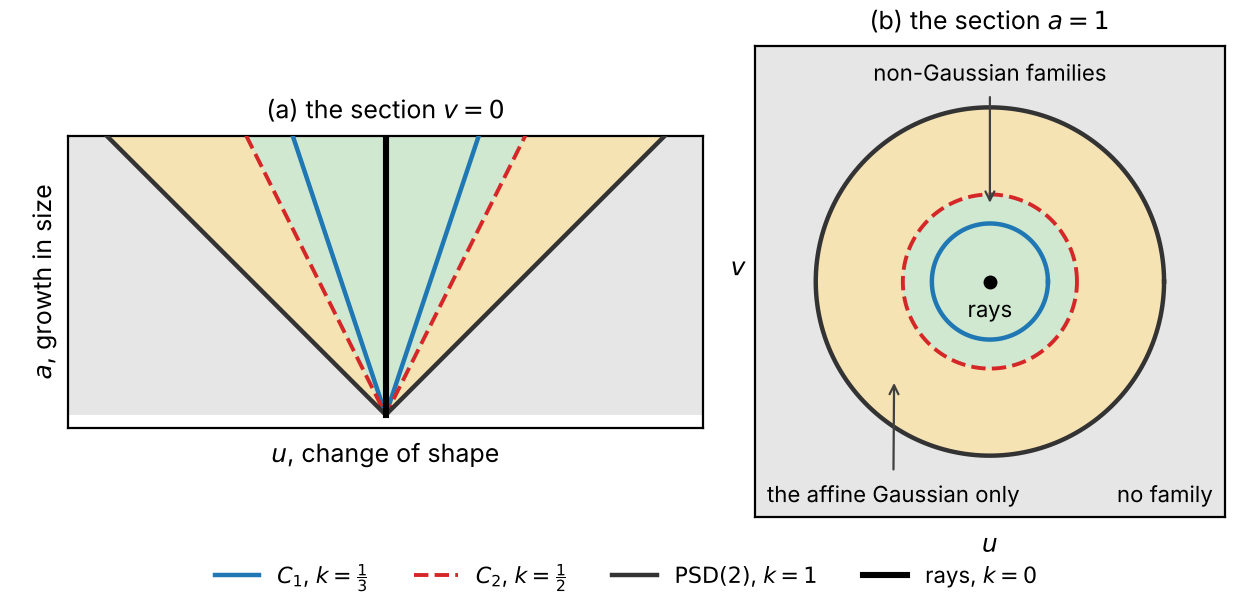
\includegraphics[width=\textwidth]{fig-cones-plane.png}
\caption{The rotation-invariant cones of velocities in the plane, in the coordinates $(a, u, v)$ of
$X = \bigl(\begin{smallmatrix} a+u & v \\ v & a-u \end{smallmatrix}\bigr)$: each is a round cone
$\sqrt{u^2+v^2} \le k\,a$ about the axis of the multiples of $I$. (a) The section $v = 0$, where each
cone is a sector. (b) The section $a = 1$, where each cone is a disc of radius $k$. Drawn are the rays
($k = 0$), the cone $C_1$ ($k = \frac13$), along whose order the orbit of the Poisson kernel cascades,
the cone $C_2$ ($k = \frac12$) and the Loewner cone $\PSD(2)$ ($k = 1$). The shading reads
Theorem~\ref{thm:wedge-axis} in the plane: a cone with $k < \frac12$ (green) carries non-Gaussian
families, one with $\frac12 \le k \le 1$ (amber) only the affine Gaussian scale spaces, and one with
$k > 1$ (grey) none. Drawn by a script deposited with the paper.}
\label{fig:cones-plane}
\end{figure}

The rest of the subsection is linear algebra, in the language of matrix analysis and of the Lie theory
of semigroups, where the orders of a homogeneous space are studied through their cones (``Prior art''
at the end of the subsection).
% Round 2 (presentation review), item 19 (VERIFY-round2-notation-paper.md § 19): the motivation of
% causal curves and of majorization, compared with Theorem 4.3(1) (the test log M in C is its
% conclusion, the order being defined by curves) and Lemma C.1(2), (5).
An order is described by its set of relative steps $M = \Sigma^{-1/2}\Sigma'\Sigma^{-1/2}$
(Proposition~\ref{prop:invariant-orders}), and an $\Orth(d)$-invariant closed convex cone $C$ of symmetric matrices plays
the part of the allowed velocities, through the cone field of Theorem~\ref{thm:cone-orders}. A single
step is tested by its logarithm: Theorem~\ref{thm:cone-orders}(1) shows that a curve of that cone
field joins $\Sigma$ to $\Sigma'$ exactly when $\log M \in C$. Steps do not compose by multiplication.
The composite of two steps $M$ and $N$ is $M^{1/2}N'M^{1/2}$ with $N'$ a rotation of $N$
(Proposition~\ref{prop:invariant-orders}(3)), and its logarithm is not $\log M + \log N'$ when $M$
and $N'$ do not commute. So it is not obvious that the test is transitive. A comparison of spectra by partial sums,
majorization, bounds the spectrum of the composite whatever the relative position of the eigenframes,
with one cited inequality (C4, Theorem~\ref{thm:cited-A9}). It gives both the transitivity and the
fact that a curve of the cone field ends at a step in $\exp C$.
Proposition~\ref{prop:invariant-orders} sets up the dictionary between invariant orders and sets of
steps in which the theorem is stated.

% shared with blueprint prop:invariant-orders
\begin{proposition}[invariant relations on $\PD(d)$ and their steps]\label{prop:invariant-orders}
Let $d \ge 1$ and write $\Sym(d)$ for the real symmetric $d \times d$ matrices. Call a set
$\mathcal K \subseteq \PD(d)$ a \emph{step set} if $QMQ^{\tp} \in \mathcal K$ whenever $M \in \mathcal K$
and $Q \in \Orth(d)$. For a step set write $\Sigma \le_{\mathcal K} \Sigma'$, for
$\Sigma, \Sigma' \in \PD(d)$, when the \emph{relative step} $\Sigma^{-1/2}\Sigma'\Sigma^{-1/2}$ lies in
$\mathcal K$, and put $\mathcal S_{\mathcal K} := \{A \in \GL(d) : AA^{\tp} \in \mathcal K\}$.
\begin{enumerate}
\item \emph{(Invariant relations are step sets.)} For $\Sigma, \Sigma' \in \PD(d)$ and every
$A \in \GL(d)$ with $AA^{\tp} = \Sigma$, $\Sigma \le_{\mathcal K} \Sigma'$ if and only if
$A^{-1}\Sigma'A^{-\tp} \in \mathcal K$. The relation $\le_{\mathcal K}$ is $\GL(d)$-invariant:
$\Sigma \le_{\mathcal K} \Sigma'$ if and only if $B\Sigma B^{\tp} \le_{\mathcal K} B\Sigma'B^{\tp}$, for
every $B \in \GL(d)$. Every $\GL(d)$-invariant relation $R$ on $\PD(d)$ is $\le_{\mathcal K}$ for
exactly one step set, $\mathcal K = \{M \in \PD(d) : I \,R\,M\}$.
\item \emph{(Order properties.)} $\le_{\mathcal K}$ is reflexive if and only if $I \in \mathcal K$; it is
antisymmetric if and only if no $M \ne I$ has both $M$ and $M^{-1}$ in $\mathcal K$; and it is closed in
$\PD(d) \times \PD(d)$ if and only if $\mathcal K$ is closed in $\PD(d)$.
\item \emph{(How steps compose.)} If $\Sigma \le_{\mathcal K} \Sigma' \le_{\mathcal K} \Sigma''$, $M$ is
the relative step of $(\Sigma, \Sigma')$ and $N$ that of $(\Sigma', \Sigma'')$, then the relative step
of $(\Sigma, \Sigma'')$ is $M^{1/2}N'M^{1/2}$ with $N' = Q^{\tp}NQ$ for some $Q \in \Orth(d)$, and its
eigenvalues are those of $MN'$. Conversely, for $M, N \in \mathcal K$ the triple $I$, $M$,
$M^{1/2}NM^{1/2}$ is such a chain. So $\le_{\mathcal K}$ is transitive if and only if
$M^{1/2}NM^{1/2} \in \mathcal K$ for all $M, N \in \mathcal K$, if and only if $\mathcal S_{\mathcal K}$
is closed under products. The spectrum of the composite is not determined by the spectra of the two
steps: for $d = 2$ the step $\diag(4,1)$ followed by $\diag(4,1)$ gives $\diag(16,1)$, and followed by
$\diag(1,4)$ gives $4I$.
\item \emph{(The infinitesimal cone.)} The set
$C(\mathcal K) := \{X \in \Sym(d) : e^{tX} \in \mathcal K \text{ for every } t \ge 0\}$ is invariant
under $X \mapsto QXQ^{\tp}$, $Q \in \Orth(d)$, and under $X \mapsto cX$, $c \ge 0$. It is closed when
$\mathcal K$ is closed in $\PD(d)$, and if $\le_{\mathcal K}$ is antisymmetric then
$X \in C(\mathcal K)$ and $-X \in C(\mathcal K)$ only for $X = 0$.
\end{enumerate}
\end{proposition}

Clause (1) is the dictionary between the orders of the scheme and sets of matrices: a
$\GL(d)$-invariant order on $\PD(d) = \GL(d)/\Orth(d)$ is its set of relative steps at $I$.
The proof is in Appendix~\ref{app:wedge-axis}.

The invariant cones are read through their eigenvalues. For $X \in \Sym(d)$ write
$\lambda^\uparrow(X)$ for its eigenvalues in increasing order, and for a cone $C \subseteq \Sym(d)$
put $\exp C := \{e^X : X \in C\}$.

An invariant cone generates an order along curves that move in the cone at each point. The theorem
says which orders arise in this way, and its clause (4) gives the orders on $\PSD(d)$ along which the
general linear row is read in \S\ref{sec:wedge-axis-proof}.

% CHANGED Q-0281 wave 2: blind review W2F-4 (the sentence above) and W2F-5 (the parenthetical of clause
% (3), mirrored from the blueprint statement).
% shared with blueprint thm:cone-orders
\begin{theorem}[invariant orders generated by cone fields]\label{thm:cone-orders}
Let $d \ge 1$ and let $C \subseteq \Sym(d)$ be a closed convex cone invariant under $X \mapsto QXQ^{\tp}$,
$Q \in \Orth(d)$. Its \emph{cone field} assigns to $\Sigma \in \PD(d)$ the cone
$\Sigma^{1/2}C\Sigma^{1/2}$ of tangent vectors, which equals $ACA^{\tp}$ for every $A$ with
$AA^{\tp} = \Sigma$, so that $B(\Sigma^{1/2}C\Sigma^{1/2})B^{\tp}$ is the cone at $B\Sigma B^{\tp}$ for
$B \in \GL(d)$. An absolutely continuous $\gamma : [0,1] \to \PD(d)$ is \emph{$C$-causal} if
$\gamma(t)^{-1/2}\gamma'(t)\gamma(t)^{-1/2} \in C$ for almost every $t$; write $\Sigma \preceq_C \Sigma'$
when a $C$-causal curve runs from $\Sigma$ to $\Sigma'$. Use the notation of Proposition~\ref{prop:invariant-orders}
(step sets $\mathcal K$, their relations $\le_{\mathcal K}$, the sets $\mathcal S_{\mathcal K}$ and the cones
$C(\mathcal K)$), write $\exp C := \{e^X : X \in C\}$, and write $\lambda^\uparrow_1(M)$ for the least
eigenvalue of $M$.
\begin{enumerate}
\item \emph{(The order of a cone field.)} $\Sigma \preceq_C \Sigma'$ if and only if the relative step
$M = \Sigma^{-1/2}\Sigma'\Sigma^{-1/2}$ lies in $\exp C$, and then $\gamma(t) := \Sigma^{1/2}M^t\Sigma^{1/2}$
is $C$-causal. So $\preceq_C$ is $\le_{\exp C}$: a closed $\GL(d)$-invariant preorder, which is a partial
order if and only if $C \cap (-C) = \{0\}$; and $C(\exp C) = C$.
\item \emph{(Closed invariant orders.)} Let $\mathcal K$ be a closed step set for which $\le_{\mathcal K}$
is a partial order. Then
$\{B \in \gl(d) : e^{tB} \in \mathcal S_{\mathcal K} \text{ for every } t \ge 0\} =
\{B : \tfrac12(B + B^{\tp}) \in C(\mathcal K)\}$, and this is a closed convex cone containing every
skew-symmetric matrix; $C(\mathcal K)$ is an $\Orth(d)$-invariant closed convex cone with
$C(\mathcal K) \cap (-C(\mathcal K)) = \{0\}$; and $\preceq_{C(\mathcal K)}$ is contained in
$\le_{\mathcal K}$. The following are equivalent: (a) $\le_{\mathcal K}$ is $\preceq_{C'}$ for some cone
$C'$ as above; (b) $\mathcal K = \exp C(\mathcal K)$; (c) $M^\tau \in \mathcal K$ whenever
$M \in \mathcal K$ and $0 \le \tau \le 1$. When they hold, $C' = C(\mathcal K)$.
\item \emph{(A closed order without a cone.)} $\mathcal K := \{I\} \cup \{M \in \PD(d) :
\lambda^\uparrow_1(M) \ge 2\}$ is a closed step set, $\le_{\mathcal K}$ is a partial order, and
$C(\mathcal K) = \{0\}$, so that $\preceq_{C(\mathcal K)}$ is equality; hence $\le_{\mathcal K}$ is
$\preceq_{C'}$ for no cone $C'$.
\item \emph{(On $\PSD(d)$.)} Suppose $I \in C$ and $C \cap (-C) = \{0\}$. For $\Sigma, \Sigma' \in
\PSD(d)$ let $\Sigma \preceq^+_C \Sigma'$ when $\Sigma = 0$, or $\Sigma' = c\,\Sigma$ for some $c \ge 1$,
or $\Sigma, \Sigma' \in \PD(d)$ and $\Sigma \preceq_C \Sigma'$. Then $\preceq^+_C$ is a $\GL(d)$-invariant
partial order on $\PSD(d)$ that contains the rays, every pair $\Sigma \preceq^+_C \Sigma'$ is joined by a
chain as in Theorem~\ref{thm:cascade-infinitely-divisible}(2), and $(G, \preceq^+_C)$ is a wedge datum with the
path condition (P) for every closed subgroup $G$ of $\GL(d)$ containing the dilations. It is contained in
the Loewner order if and only if $C \subseteq \PSD(d)$. For $C = \{cI : c \ge 0\}$ it is the ray order of
Definition~\ref{def:gw-cascade-family}.
\end{enumerate}
\end{theorem}

So an $\Orth(d)$-invariant closed convex cone generates an invariant preorder whose steps are exactly
the exponentials of the cone, and a partial order when $C \cap (-C) = \{0\}$. The steps are reached along the geodesics $\Sigma^{1/2}M^t\Sigma^{1/2}$, and
no closure is needed. A closed invariant order comes from a cone exactly when its steps are closed
under fractional powers, and clause (3) shows that the restriction is needed: a closed invariant
order can have no infinitesimal part at all. At $C = \PSD(d)$, clause (4) adds to the Loewner order of
$\PD(d)$ only the origin and the rays. It is therefore smaller than the Loewner order of $\PSD(d)$,
which also has steps from nonzero singular matrices to definite ones. The proof, in
Appendix~\ref{app:wedge-axis}, runs through one family of functionals, which
Lemma~\ref{lem:spectral-cones} makes superadditive along any three points.

A vector $x \in \RR^d$ is \emph{majorized} by $y$ when, for every $k$, the sum of the $k$ smallest
entries of $x$ is at least that of $y$, with equal totals: $x$ is the less spread of the two.
% Round 3 (content review), C-S3: Bhatia states (III.21) through the largest entries.
The source of C4 states its inequality in the equivalent form of partial sums of the largest entries
(\S\ref{sec:cited-facts}). Two matrix inequalities
carry the correspondence. The eigenvalues of a sum $X + Y$ are majorized by the sum of the two
spectra, and the logarithmic spectrum of a product $M^{1/2}NM^{1/2}$ by the sum of the logarithmic
spectra of $M$ and $N$. Clause (3) of Proposition~\ref{prop:invariant-orders} is the reason
majorization is the tool here: the spectrum of a composite is not a function of the two spectra, but
majorization bounds it uniformly over the rotation between the eigenframes.
Lemma~\ref{lem:spectral-cones} states the two inequalities, proves the first, and derives the second
from the cited fact C4 and a determinant, with the description of the $\Orth(d)$-invariant closed
convex cones by symmetric cones of eigenvalues and the transitivity of $\le_{\exp C}$. It is in
Appendix~\ref{app:wedge-axis}, with the proofs it serves.

The cones that matter here form one chain, from the rays to the Loewner order:
$C_\alpha := \{X \in \PSD(d) : (d+\alpha)\,\lambda_{\min}(X) \ge \tr X\}$ for $0 \le \alpha < \infty$, and
$C_\infty := \PSD(d)$. Its members of index $0 < \alpha < 2$ are the symmetric parts of the exponent
cones of the stable laws, and Proposition~\ref{prop:stable-order-generated} in \S\ref{sec:affine-stable-cone} shows that
their orders are the stable orders.

\paragraph{Prior art.} The correspondence between invariant cone fields, Lie wedges, semigroups and
closed orders on a homogeneous space $G/H$ is Lawson's (\sscite{lawson1989ordered}, Thm.~4.9, p.~290;
Props.~6.3--6.4, pp.~295--296; Thms.~7.4--7.5, pp.~300--302), on the Lie theory of semigroups of
Hilgert, Hofmann and Lawson (\sscite{hilgert1989lie}, Prop.~V.1.7, pp.~375--376). Read on $\GL(d)$
with the involution $A \mapsto A^{-\tp}$, their Cor.~V.4.58 (p.~440) gives the transitivity of
Theorem~\ref{thm:cone-orders}(1) for pointed cones, and their abelian example (p.~376) is the model of
Theorem~\ref{thm:cone-orders}(3). Hilgert and \'Olafsson state the bijection between invariant regular
cones and invariant regular causal structures (\sscite{hilgert1997causal}, Thm.~2.2.2, p.~40), and the dual
description of a closed convex cone is in Faraut and Kor\'anyi (\sscite{faraut1994analysis},
Thm.~I.1.1, p.~2).
% Round 3 (content review), C-R4, D-R7 (VERIFY-round3-landscape-orbits-paper.md item 11; the author's
% decision D13): no priority claim. "Which is not connected" dropped, the powers-versus-roots reason
% kept. Lawson 1994 acquired and read at the page (D13; records/affine/READING-lawson1994polar.md): his
% Thm. 3.1 has the closedness and the wedges that are not pointed, so the former contrast with Cor. V.4.58
% ("needs no closure ... the cones need not be pointed") went. Hilgert-Neeb 1993, Neeb 2000 and Kostant are
% not held, and nothing is said against them.
Here the correspondence is read on $\PD(d)$ through step sets and their spectra and proved by
majorization. The semigroup is in Lawson's paper on polar decompositions, which allows cones that are
not pointed and derives the closedness that Cor.~V.4.58 asks for: $\mathcal S_{\exp C} = (\exp C)\Orth(d)$ is a
closed semigroup with subtangent wedge $C \oplus \mathfrak{so}(d)$, by his Thm.~3.1
(\sscite{lawson1994polar}, pp.~198--199), as $\operatorname{ad}X$ has real spectrum for symmetric $X$ (his
Lem.~4.1 and Example~4.2, p.~203) and the centre of $\gl(d)$ is $\RR I$, which gives his condition (4). By
Proposition~\ref{prop:invariant-orders}(3) that is the transitivity of $\le_{\exp C}$. His paper has no order on the quotient. The characterization by powers is the
form on $\PD(d)$ of their theorem that a closed subsemigroup of a connected Lie group is divisible,
with roots of every order, exactly when it is the exponential image of its tangent wedge, the
set of generators of the one-parameter semigroups it contains
(\sscite{hilgert1989lie}, Thm.~V.6.5, p.~460). Their divisibility asks for roots of the elements of
$\mathcal S_{\mathcal K}$, while the powers in (c) are those of the positive definite steps. The two agree
only on the symmetric elements. The proof here is by majorization. As orders, the stable
orders are the Loewner order in other coordinates (Proposition~\ref{prop:stable-order-generated}(3)), and
this paper reads them as the orders of the stable orbits (Proposition~\ref{prop:stable-step-cone}).

% §5.5 The base, and §5.6 the wedge of an orbit --- blueprint chapter 5, part 05-orbits.tex (Q-0288).
% Included from 05-landscape.tex; the conventions are in that file's header. Order: the blueprint's.
% The stable rung comes first in 5.6 because prop:orbit-step-cone reads prop:stable-step-cone;
% prop:stable-order-generated (blueprint part 05-wedges) follows prop:stable-exponent-cone, whose cone
% it reads (Q-0290, review flag S12). The two Matern cross-shape nodes and the grid remark are in
% appendix B, three routine proofs in appendix E (Q-0290). The six [A] nodes all rest on A3(iii),
% named once at the start of 5.6 (the review's length judgement). The identification of the Matern
% orbit with the anisotropic Matern of spatial statistics is a
% naming read at the page (records/affine/READING-whittle1954stationary.md,
% READING-lindgren2011explicit.md), not a fact a proof rests on.

\subsection{The base: the general linear group along rays}\label{sec:affine-orbits}

The smallest order of the scheme is the ray order. It requires only that the record at
$\lambda^2\Sigma$, $\lambda > 1$, be a further smoothing of the record at $\Sigma$: a zoom out without
a change of shape. This subsection asks which kernels can then be carried to every elliptical aperture
covariantly under the whole general linear group, and the answer is that this costs nothing beyond
what the isotropic theory requires. The kernel $\mu_I$ at the round aperture fixes the family, which is
its \emph{affine orbit}: the kernel at $\Sigma$ is $(\Sigma^{1/2})_*\mu_I$, the round kernel stretched
by $\Sigma^{1/2}$, as the Gaussian of covariance $2b\Sigma$ is the round Gaussian of covariance $2bI$
stretched. The orbit is a family along the rays exactly when $\mu_I$ is rotation invariant and
self-decomposable \ref{eq:self-decomposable} (Proposition~\ref{prop:ray-families}). The
rotation-invariant self-decomposable laws other than $\delta_0$ are the kernels from scale zero of the
isotropic families (Theorem~\ref{thm:isotropic-classification} and
Lemma~\ref{lem:radial-marginal}(1)), so every isotropic scale space, the stable and the \Matern{} ones
among them, has an affine orbit along the rays. What a non-Gaussian orbit cannot do is cascade along a
step that widens the aperture in some directions and not in others, a step of rank below $d$
(Proposition~\ref{prop:affine-orbits}(3)). The \Matern{} orbit of
Proposition~\ref{prop:affine-orbits}(4) is the example to keep in mind.

% shared with blueprint prop:affine-orbits
\begin{proposition}[affine orbits of isotropic laws]\label{prop:affine-orbits}
Let $d \ge 1$ and let $g : [0,\infty) \to [0,\infty)$ be continuous with $g(0) = 0$ and such that
$\omega \mapsto e^{-g(|\omega|^2)}$ is the characteristic function of a probability measure
$\mu_I$ on $\RR^d$. For $\Sigma \in \PD(d)$ put $\mu_\Sigma := (\Sigma^{1/2})_*\mu_I$, the
\emph{affine orbit} of $\mu_I$.
\begin{enumerate}
\item \emph{(Covariance.)} $\widehat\mu_\Sigma(\omega) = e^{-g(\langle\omega,\Sigma\omega\rangle)}$,
and $A_*\mu_\Sigma = \mu_{A\Sigma A^{\tp}}$ for every $A \in \GL(d)$ and $\Sigma \in \PD(d)$.
\item \emph{(Cascade along rays.)} If for some $\lambda > 1$ there is a probability measure
$\nu_\lambda$ on $\RR^d$ with $e^{-g(\lambda^2|\omega|^2)} = e^{-g(|\omega|^2)}\,\widehat\nu_\lambda(\omega)$,
then $\mu_{\lambda^2\Sigma} = \mu_\Sigma * (\Sigma^{1/2})_*\nu_\lambda$ for every
$\Sigma \in \PD(d)$.
\item \emph{(No cascade across shapes.)} If $d \ge 2$ and $g$ is not linear, then for no
$\Sigma \in \PD(d)$ and no $P \in \PSD(d)$ with $0 < \rank P < d$ is
$\mu_{\Sigma+P} = \mu_\Sigma * \rho$ with $\rho$ a probability measure. In particular the orbit is
not the family of kernels from scale zero of any affine cascade family.
\item \emph{(The \Matern{} orbits.)} For $\gamma > 0$, $g_\gamma(u) := \gamma\log(1+u)$ satisfies
the hypothesis in every dimension: $(1+|\omega|^2)^{-\gamma}$ is the characteristic function of
the law of $\sqrt{2V}\,Z$, with $V$ Gamma distributed of shape $\gamma$ and scale $1$ and $Z$
standard normal on $\RR^d$, independent. Its orbit has
$\widehat\mu_\Sigma(\omega) = (1 + \langle\omega,\Sigma\omega\rangle)^{-\gamma}$; clause (3)
applies to it, $g_\gamma$ not being linear; and the hypothesis of clause (2) holds for every
$\gamma > 0$ and every $\lambda > 1$, with $\nu_\lambda$ the law of $\sqrt{2Y}\,Z$, where $Z$ is
standard normal on $\RR^d$ and $Y \ge 0$, independent of $Z$, is compound Poisson with \Levy{}
measure $\gamma\,(e^{-x/\lambda^2} - e^{-x})\,x^{-1}dx$ on $(0,\infty)$, of total mass
$2\gamma\log\lambda$.
\end{enumerate}
\end{proposition}

Clause (3) is Theorem~\ref{thm:rank-deficient-step} read on the orbit. The stable orbit
$e^{-\langle\omega,\Sigma\omega\rangle^{\alpha/2}}$, $0 < \alpha < 2$, is another instance of the
proposition (Lemma~\ref{lem:elliptical-stable}), so by clause (3) it is not a family along the Loewner
order. For $\gamma > d/2$ the family of clause (4) is the \Matern{} covariance of spatial statistics
(\sscite{matern1960spatial}, (2.4.5)--(2.4.7), pp.~17--18; \sscite{whittle1954stationary}, \S9,
pp.~447--448; \sscite{lindgren2011explicit}, \S2.1, eqs.~(1)--(2), p.~426), with geometric anisotropy
(\sscite{lindgren2011explicit}, \S3.4, p.~437), in which the matrix is a parameter of the covariance. Clause (3) excludes
the rank-deficient steps between two values of it, and Proposition~\ref{prop:matern-steps} shows that
no step across shapes has a positive increment.
The proof is in Appendix~\ref{app:proofs}.


The converse holds: a family covariant under the general linear group that cascades along the ray of
$I$ is such an orbit, and the law must be self-decomposable.

% shared with blueprint prop:ray-families+663841edc318
\begin{proposition}[the ray families are the orbits of the self-decomposable isotropic laws]\label{prop:ray-families}
Let $d \ge 1$ and let $(\mu_\Sigma)_{\Sigma\in\PD(d)}$ be probability measures on $\RR^d$ with
\begin{enumerate}
\item[(R1)] \emph{(affine covariance)} $A_*\mu_\Sigma = \mu_{A\Sigma A^{\tp}}$ for every
$A \in \GL(d)$ and $\Sigma \in \PD(d)$;
\item[(R2)] \emph{(a cascade along the ray of $I$)} for every $\lambda > 1$ there is a probability
measure $\rho_\lambda$ on $\RR^d$ with $\mu_{\lambda^2I} = \mu_I * \rho_\lambda$.
\end{enumerate}
Then $\mu_I$ is rotation invariant and self-decomposable \ref{eq:self-decomposable},
$\mu_\Sigma = (\Sigma^{1/2})_*\mu_I$ for every $\Sigma$, and the family cascades along every ray:
$\mu_{\lambda^2\Sigma} = \mu_\Sigma * (\Sigma^{1/2})_*\rho_\lambda$ for every $\Sigma \in \PD(d)$
and $\lambda > 1$. Conversely, for every rotation-invariant self-decomposable law $\mu_I$ on
$\RR^d$ the family $\mu_\Sigma := (\Sigma^{1/2})_*\mu_I$ satisfies (R1) and (R2).
\end{proposition}

With Theorem~\ref{thm:affine-rigidity} this places the obstruction for $d \ge 2$: along the rays every
rotation-invariant self-decomposable law keeps its orbit, and across every step of the Loewner order
only the Gaussian does. Which steps across shapes
an orbit survives depends on the law, and that is the next subsection.

% proof of prop:ray-families
\begin{proof}
(R1) is (K3) of Definition~\ref{def:affine-cascade-family} for the kernels from scale zero, and (R2)
is (K1) along the ray of $I$ alone.

\emph{Covariance determines the orbit.} (R1) with $A = Q \in \Orth(d)$ and $\Sigma = I$ gives
$Q_*\mu_I = \mu_{QQ^{\tp}} = \mu_I$, and with $A = \Sigma^{1/2}$ it gives
$(\Sigma^{1/2})_*\mu_I = \mu_\Sigma$, as for the orbits of Proposition~\ref{prop:affine-orbits}.

\emph{Self-decomposability.} By (R1) with $A = \lambda I$, $\mu_{\lambda^2I} = (\lambda I)_*\mu_I$,
so (R2) reads $(\lambda I)_*\mu_I = \mu_I * \rho_\lambda$. Applying $(\lambda^{-1}I)_*$ gives
$\mu_I = (cI)_*\mu_I * (cI)_*\rho_\lambda$ with $c := \lambda^{-1}$, which is
\ref{eq:self-decomposable} with the residual $(cI)_*\rho_\lambda$, and every $c \in (0,1)$ arises.

\emph{Every ray.} $\mu_{\lambda^2\Sigma} = (\Sigma^{1/2})_*\mu_{\lambda^2I}
= (\Sigma^{1/2})_*(\mu_I * \rho_\lambda) = \mu_\Sigma * (\Sigma^{1/2})_*\rho_\lambda$.

\emph{Converse.} For (R1), let $B := A\Sigma^{1/2}$ and $\Sigma' := A\Sigma A^{\tp} = BB^{\tp}$. Then
$Q := \Sigma'^{-1/2}B$ is orthogonal, so
$A_*\mu_\Sigma = B_*\mu_I = (\Sigma'^{1/2})_*Q_*\mu_I = \mu_{\Sigma'}$. For (R2), self-decomposability
at $c := \lambda^{-1}$ gives $\mu_I = (cI)_*\mu_I * \rho_c$, and applying $(\lambda I)_*$ gives
$\mu_{\lambda^2I} = \mu_I * (\lambda I)_*\rho_c$.
\end{proof}

\subsection{The step set of an orbit}\label{sec:affine-stable-cone}

Shape adaptation changes the shape of the aperture as the scale grows (\S\ref{sec:landscape-uses}, the third use).
For the Gaussian every Loewner step is a further smoothing, so the shape may change as fast as
Lemma~\ref{lem:loewner-scale-shape}(3) allows: in the plane, a step that doubles the volume scale
reaches an anisotropy gained of $4$ and no more. This subsection asks the same of the other affine
orbits. Along which steps $\Sigma \to \Sigma'$ across shapes is the kernel at $\Sigma'$ the kernel at
$\Sigma$ convolved with a probability measure? Along those steps the coarser record is a further
smoothing of the finer one, and along every other step a change of shape is a re-measurement of the
image.

To state the question for every orbit, relate two apertures $\Sigma, \Sigma' \in \PD(d)$
when $\mu_{\Sigma'} = \mu_\Sigma * \rho$ for a positive finite measure $\rho$. The orbit is covariant
under $\GL(d)$ (Proposition~\ref{prop:affine-orbits}(1)), so this relation is $\GL(d)$-invariant, and by
Proposition~\ref{prop:invariant-orders}(1) it is $\le_{\mathcal K}$ for exactly one step set
$\mathcal K$: the set of $M$ with $\mu_M = \mu_I * \rho$. Call $\mathcal K$ the \emph{step set} of the
orbit. It contains the rays exactly when $\mu_I$ is self-decomposable
(Proposition~\ref{prop:ray-families}). For a non-Gaussian orbit it contains no step
$\Sigma \to \Sigma + P$ with $0 < \rank P < d$ (Proposition~\ref{prop:affine-orbits}(3)), so the
question is about steps of full rank.

The answer depends on the kernel. The orbit of the isotropic $\alpha$-stable law, $0 < \alpha < 2$,
cascades on full-rank steps of every orientation, under a speed limit of the Gaussian's form and
narrower: with $t_1, t_2$ the volume scales of the two apertures, the anisotropy gained is at most
$(t_2/t_1)^{d\alpha/(d+\alpha)}$, against $(t_2/t_1)^d$ for the Gaussian
(Proposition~\ref{prop:stable-step-cone}(3) and Lemma~\ref{lem:loewner-scale-shape}(3)). For the
Poisson kernel, $\alpha = 1$ (\S\ref{sec:classical-prior-art}), a step in the plane that doubles the
volume scale reaches an anisotropy gained of $2^{2/3} \approx 1.59$ and no more, and
Figure~\ref{fig:shape-plane} draws both limits. At the other end, the \Matern{} orbits cascade along
the rays and along no other step (Proposition~\ref{prop:matern-steps}). No orbit whose transform falls
off like a power of the frequency, in the sense of Proposition~\ref{prop:log-orbit-rays}, has a
positive increment on a step off the rays, and the orbits of decaying rational symbols are among them
(Proposition~\ref{prop:rational-symbols}). For the orbit of a general profile, one function of the
profile, its dilation ratio, gives a set of steps on which the orbit cascades
(Proposition~\ref{prop:orbit-step-cone}); whether it cascades on more steps is open. The subsection
ends with what the theorem on the general linear row (\S\ref{sec:wedge-axis-proof}) takes from the
orbits: the exponents of the isotropic stable law, the bound they put on a non-Gaussian law, and the
stable order extended to $\PSD(d)$.

The answers are read through the \Levy--Khintchine representation (C2, Theorem~\ref{thm:cited-A3}),
and from here on the subsection uses its vocabulary. The kernels of the stable orbits and of the
orbits of Proposition~\ref{prop:orbit-step-cone} are \emph{infinitely divisible} laws with no
Gaussian part. Each is the law of a sum of independent displacements, and its \emph{\Levy{} measure}
gives the expected number of displacements of each size and direction. Here that measure has a
density $n_\Sigma(x)$, the rate of the displacements per unit volume, not the density of the kernel.
A step $\Sigma \to \Sigma'$ is a further smoothing when the kernel at $\Sigma'$ has at least the rate
of displacements of the kernel at $\Sigma$ at every size and in every direction,
$n_\Sigma \le n_{\Sigma'}$ (Proposition~\ref{prop:orbit-step-cone}(2)), and for the stable orbits only
then (Proposition~\ref{prop:stable-step-cone}(1)).

\subsubsection*{The stable rung}

The chain of cones $C_\alpha$ of \S\ref{sec:invariant-wedges} is a ladder from the rays ($\alpha = 0$)
to the Loewner order ($\alpha = \infty$). Call the \emph{rung} of an orbit the largest index $\alpha$
whose stable order its step set contains. The elliptical stable laws are built from their \Levy{}
densities.

% shared with blueprint lem:elliptical-stable
\begin{lemma}[the elliptical stable laws]\label{lem:elliptical-stable}
Let $d \ge 1$ and $0 < \alpha < 2$, and put
\[
  c_{d,\alpha} := \int_{\RR^d}(1 - \cos y_1)\,|y|^{-d-\alpha}\,dy .
\]
Then $0 < c_{d,\alpha} < \infty$. For $H \in \PD(d)$ and $x \in \RR^d \setminus \{0\}$ put
\begin{equation}\label{eq:stable-levy-density}
  n_H(x) := c_{d,\alpha}^{-1}(\det H)^{-1/2}\langle x,H^{-1}x\rangle^{-(d+\alpha)/2} ,
  \qquad \psi_H(\omega) := \langle\omega,H\omega\rangle^{\alpha/2} .
\end{equation}
\begin{enumerate}
\item For every $H \in \PD(d)$ and $\omega \in \RR^d$,
$\psi_H(\omega) = \int_{\RR^d\setminus\{0\}}(1 - \cos\langle\omega,x\rangle)\,n_H(x)\,dx$, and
$\int_{\RR^d\setminus\{0\}}(|x|^2 \wedge 1)\,n_H(x)\,dx < \infty$.
\item For every $H \in \PD(d)$ there is a unique probability measure $S_\alpha(H)$ on $\RR^d$ with
$\widehat{S_\alpha(H)} = e^{-\psi_H}$. It is infinitely divisible with generating triplet
$(0, n_H(x)\,dx, 0)$, and $A_*S_\alpha(H) = S_\alpha(AHA^{\tp})$ for every $A \in \GL(d)$.
\item $n_{AHA^{\tp}}(x) = |\det A|^{-1}\,n_H(A^{-1}x)$ for $A \in \GL(d)$, $H \in \PD(d)$ and
$x \ne 0$.
\end{enumerate}
In particular $g(u) := u^{\alpha/2}$ satisfies the hypothesis of Proposition~\ref{prop:affine-orbits}, with
$\mu_I = S_\alpha(I)$, and the affine orbit of $S_\alpha(I)$ is $\mu_\Sigma = S_\alpha(\Sigma)$, the
\emph{stable orbit}.
\end{lemma}

The law $S_\alpha(H)$ is the rotation-invariant $\alpha$-stable law (\sscite{sato1999levy}, Thm.~14.14,
p.~86) transported by $H^{1/2}$, with its constant normalized to $1$. In the terms of Samorodnitsky
and Taqqu it is a sub-Gaussian stable law. The existence in (2) is their Proposition~2.5.2 with
$R = 2H$, and their Proposition~2.5.7 makes every such law a linear image of $S_\alpha(I)$
(\sscite{samorodnitsky1994stable}, pp.~78 and~81). At $\alpha = 1$, $S_1(I)$ is the kernel of the Poisson scale
space at unit scale, with transform $e^{-|\omega|}$ (\S\ref{sec:classical-prior-art}). The proof is in
Appendix~\ref{app:proofs}.

The stable orbit cascades on a cone of full-rank steps, the steps whose \Levy{} densities
\ref{eq:stable-levy-density} are ordered.

% shared with blueprint prop:stable-step-cone+2382c75d66ad
\begin{proposition}[the stable orbit cascades on a cone of full-rank steps]\label{prop:stable-step-cone}
Let $d \ge 1$, $0 < \alpha < 2$, and let $\mu_\Sigma = S_\alpha(\Sigma)$, $\Sigma \in \PD(d)$, be the
stable orbit (Lemma~\ref{lem:elliptical-stable}). For $\Sigma, \Sigma' \in \PD(d)$ put
$M := \Sigma^{-1/2}\Sigma'\Sigma^{-1/2}$ and let $\lambda_{\min}(M)$ be its least eigenvalue.
\begin{enumerate}
\item \emph{(The step cone.)} The following are equivalent:
(a) there is a positive finite measure $\rho$ with $\mu_{\Sigma'} = \mu_\Sigma * \rho$;
(b) $n_\Sigma(x) \le n_{\Sigma'}(x)$ for every $x \ne 0$;
(c) $\lambda_{\min}(M)^{d+\alpha} \ge \det M$.
When they hold, $\Sigma \le \Sigma'$, and $\rho$ is unique: it is the infinitely divisible probability
measure $\rho_{\Sigma,\Sigma'}$ with generating triplet $(0, (n_{\Sigma'} - n_\Sigma)(x)\,dx, 0)$.
\item \emph{(The order.)} Write $\Sigma \preceq_\alpha \Sigma'$ when (c) holds. This is a partial order
on $\PD(d)$, contained in the Loewner order, and $\Sigma \preceq_\alpha \Sigma'$ if and only if
$A\Sigma A^{\tp} \preceq_\alpha A\Sigma'A^{\tp}$, for every $A \in \GL(d)$. The increments satisfy
$\rho_{\Sigma,\Sigma} = \delta_0$, $\rho_{\Sigma,\Sigma''} = \rho_{\Sigma',\Sigma''} * \rho_{\Sigma,\Sigma'}$
whenever $\Sigma \preceq_\alpha \Sigma' \preceq_\alpha \Sigma''$, and
$A_*\rho_{\Sigma,\Sigma'} = \rho_{A\Sigma A^{\tp},A\Sigma'A^{\tp}}$.
\item \emph{(Which steps.)} Every ray, $\Sigma' = \lambda^2\Sigma$ with $\lambda \ge 1$, satisfies
$\Sigma \preceq_\alpha \Sigma'$, and no step $\Sigma' = \Sigma + P$ with $P \in \PSD(d)$ and
$0 < \rank P < d$ does. In the coordinates of Lemma~\ref{lem:loewner-scale-shape} (volume scales $t_1, t_2$,
the eigenvalues $n_1 \le \dots \le n_d$ of the relative shape $N$),
\[
  \Sigma_1 \preceq_\alpha \Sigma_2 \Longleftrightarrow n_1 \ge (t_1/t_2)^{2\alpha/(d+\alpha)} ,
\]
so the anisotropy gained, $\sqrt{n_d/n_1}$, is at most $(t_2/t_1)^{d\alpha/(d+\alpha)}$; and for
every $t_2 \ge t_1$ and every $N \in \PD(d)$ with $\det N = 1$ and least eigenvalue at least
$(t_1/t_2)^{2\alpha/(d+\alpha)}$, the matrix $\Sigma_2 := t_2^2S_1^{1/2}NS_1^{1/2}$ satisfies
$\Sigma_1 \preceq_\alpha \Sigma_2$. In particular, for $d \ge 2$ and $t_2 > t_1$ the relative shape
of a step in the cone may be any $N \ne I$ in that range, with any eigenvectors.
\end{enumerate}
\end{proposition}

So the stable orbits, which are not Gaussian, cascade across shapes, on full-rank steps of every
orientation. What
limits a step is its relative anisotropy, the gap between $\lambda_{\min}(M)$ and the geometric mean
$(\det M)^{1/d}$, and not its orientation. The cone lies between the rays and the Loewner order: the
Loewner order is $n_1 \ge (t_1/t_2)^2$ (Lemma~\ref{lem:loewner-scale-shape}(1)). Clause (3)
excludes the steps of rank below $d$ by condition (c), as Theorem~\ref{thm:rank-deficient-step} does for
$g(u) = u^{\alpha/2}$. By Proposition~\ref{prop:stable-order-generated}(1) the order is that of the
cone field $C_\alpha$.

The proof of (a)$\Rightarrow$(b) rests on a lemma that reads the \Levy{} densities off the tail of an
increment. Positivity is tested against functions supported at a large scale, so only a weak form of
the tail is needed, and the homogeneity of the exponent gives it.

% shared with blueprint lem:stable-tail
\begin{lemma}[the tail of an increment is the difference of the \Levy{} densities]\label{lem:stable-tail}
Let $d \ge 1$, $0 < \alpha < 2$, $H, H' \in \PD(d)$, and $C$ a real $d \times d$ matrix.
Suppose $\rho$ is a positive finite measure on $\RR^d$ with
\begin{equation}\label{eq:stable-tail-transform}
  \widehat\rho(\omega) = \exp\bigl[-\langle\omega,C\omega\rangle - \psi_{H'}(\omega) + \psi_H(\omega)\bigr]
  \qquad (\omega \in \RR^d),
\end{equation}
with $\psi_H$ and $n_H$ as in \ref{eq:stable-levy-density}. Then $\rho$ is a probability measure,
and for every smooth $\phi$ with compact support in $\RR^d \setminus \{0\}$
\begin{equation}\label{eq:stable-tail}
  \lim_{R\to\infty} R^\alpha\int\phi(x/R)\,\rho(dx) = \int\phi(x)\,\bigl(n_{H'}(x) - n_H(x)\bigr)\,dx .
\end{equation}
Consequently $n_H(x) \le n_{H'}(x)$ for every $x \ne 0$.
\end{lemma}

Since $n_{H'} - n_H$ is homogeneous of degree $-d-\alpha$, the right-hand side of \ref{eq:stable-tail}
equals $R^\alpha\int\phi(x/R)(n_{H'} - n_H)(x)\,dx$ for every $R$: at large scales the increment's mass
is that of the signed difference of \Levy{} densities. The limit compares masses at large scales, not
densities. The Gaussian factor $\langle\omega,C\omega\rangle$ is there for
Proposition~\ref{prop:similarity-stable-order-kernels}(3).

The proof writes $\int\phi(x/R)\,\rho(dx)$ by Fourier inversion as an integral of $\widehat\phi$ against
$e^{-E(\cdot/R)} - 1$, with $\widehat\rho = e^{-E}$; the term $1$ costs nothing because $\phi$ vanishes
at the origin. As the non-Gaussian part of the exponent is homogeneous of degree $\alpha$ and its Gaussian part of
degree $2 > \alpha$, the factor $R^\alpha$ turns this into $\int\phi\,(n_{H'} - n_H)\,dx$ in the limit, and a nonnegative bump supported where
$n_{H'} < n_H$ would make it negative. The complete proof is in Appendix~\ref{app:wedge-axis}.

% proof of prop:stable-step-cone
\begin{proof}
\emph{(b)$\Leftrightarrow$(c).} Substitute $x = \Sigma^{1/2}y$. Then
$\langle x,\Sigma^{-1}x\rangle = |y|^2$, $\langle x,\Sigma'^{-1}x\rangle = \langle y,M^{-1}y\rangle$ and
$\det\Sigma'/\det\Sigma = \det M$, so (b) says $\langle y,M^{-1}y\rangle/|y|^2 \le
(\det M)^{-1/(d+\alpha)}$ for every $y \ne 0$. The supremum of the left-hand side is $1/\lambda_{\min}(M)$,
so (b) is (c).

\emph{(c) gives $\Sigma \le \Sigma'$.} $\det M \ge \lambda_{\min}(M)^d$, so (c) gives $\lambda_{\min}(M) \ge 1$,
hence $M \ge I$ and $\Sigma' - \Sigma = \Sigma^{1/2}(M - I)\Sigma^{1/2} \ge 0$.

\emph{(a)$\Rightarrow$(b).} $e^{-\psi_\Sigma}$ has no zero, so
$\widehat\rho = e^{-\psi_{\Sigma'} + \psi_\Sigma}$, which is \ref{eq:stable-tail-transform} with $C = 0$,
and Lemma~\ref{lem:stable-tail} gives (b). The same identity shows that $\rho$ is unique.

\emph{(b)$\Rightarrow$(a).} $f := n_{\Sigma'} - n_\Sigma$ is nonnegative, even and at most $n_{\Sigma'}$,
so by Lemma~\ref{lem:elliptical-stable}(1) and C2(iii) there is an infinitely divisible $\rho$ with
triplet $(0, f(x)\,dx, 0)$ and $\widehat\rho = e^{-\psi_{\Sigma'} + \psi_\Sigma}$. So
$\mu_\Sigma * \rho$ and $\mu_{\Sigma'}$ have the same transform.

\emph{Clause (2).} Transitivity is that of (b), antisymmetry that of the Loewner order, and by
Lemma~\ref{lem:elliptical-stable}(3) condition (b) for $(A\Sigma A^{\tp}, A\Sigma'A^{\tp})$ is (b) for
$(\Sigma, \Sigma')$ at $A^{-1}x$. The transforms $e^{-\psi_{\Sigma'} + \psi_\Sigma}$ telescope, which
gives the cascade, and $\psi_\Sigma(A^{\tp}\omega) = \psi_{A\Sigma A^{\tp}}(\omega)$ gives the
covariance.

\emph{Clause (3).} A ray has $M = \lambda^2I$, and (c) reads $\lambda^{2(d+\alpha)} \ge \lambda^{2d}$. For
$0 < \rank P < d$, $M = I + \Sigma^{-1/2}P\Sigma^{-1/2}$ has the eigenvalue $1$ and one above $1$, so
$\lambda_{\min}(M) = 1 < \det M$. In the coordinates of Lemma~\ref{lem:loewner-scale-shape},
$M = (t_2/t_1)^2N$, so (c) is $n_1^{d+\alpha} \ge (t_1/t_2)^{2\alpha}$, and
$n_d/n_1 \le n_1^{-d} \le (t_2/t_1)^{2d\alpha/(d+\alpha)}$. The converse is
Lemma~\ref{lem:loewner-scale-shape}(3). For the last sentence take
$N = Q\diag(a, a^{-1/(d-1)}, \dots, a^{-1/(d-1)})Q^{\tp}$ with $Q$ arbitrary and
$(t_1/t_2)^{2\alpha/(d+\alpha)} \le a < 1$.
\end{proof}

\begin{remark}[a second route to (a)$\Rightarrow$(b)]\label{rem:stable-step-sato}
The implication (a)$\Rightarrow$(b) of Proposition~\ref{prop:stable-step-cone}(1) also follows from the
uniqueness of the generating triplet. The increment $\rho$ has the transform $e^{-E}$ with
$E := \psi_{\Sigma'} - \psi_\Sigma$, which is homogeneous of degree $\alpha$. So the image of $\rho$
under $x \mapsto n^{-1/\alpha}x$ is an $n$-th convolution root of $\rho$ for every $n$, and $\rho$ is
infinitely divisible. The generating triplets of $\mu_\Sigma$ and $\rho$ then add to one of
$\mu_{\Sigma'}$. By the uniqueness of the triplet (\sscite{sato1999levy}, Thm.~8.1(ii), pp.~37--38) the
\Levy{} measure of $\rho$ is $(n_{\Sigma'} - n_\Sigma)(x)\,dx$. So $n_{\Sigma'} - n_\Sigma \ge 0$
almost everywhere, and by continuity at every $x \ne 0$.
\end{remark}

The theorem on the general linear row needs a bound on how anisotropic the exponents of a
rotation-invariant non-Gaussian law can be. A law is \emph{operator-self-decomposable} with exponent
$B$ when it is its own image under $e^{-tB}$ convolved with a residual, for every $t > 0$
(\S\ref{sec:cited-facts}). Applying $(e^{tB})_*$, this says that the law stretched by $e^{tB}$ is the
law convolved with a probability measure, a further smoothing. For $B = I$ the stretch is a zoom, and
the condition is self-decomposability \ref{eq:self-decomposable}. On an affine orbit the kernel at $I$
stretched by $e^{tB}$ is the kernel at $e^{tB}e^{tB^{\tp}}$ (Proposition~\ref{prop:affine-orbits}(1)),
so an exponent of $\mu_I$ is a direction in which the orbit leaves the round aperture along further
smoothings. The stable law gives the bound, and for a single linear flow $e^{tB}$ the same computation
gives the set of its exponents.

% shared with blueprint prop:stable-exponent-cone+9fbc223a4e90
\begin{proposition}[the exponent cone of the isotropic stable law]\label{prop:stable-exponent-cone}
Let $d \ge 1$ and $B$ a real $d \times d$ matrix, and write $\mathrm{sym}\,B := \tfrac12(B + B^{\tp})$.
Call a probability measure $\mu$ on $\RR^d$ \emph{$B$-self-decomposable} if for every $t > 0$ there is a
probability measure $\rho_t$ with $\mu = (e^{-tB})_*\mu * \rho_t$. For $0 < \alpha < 2$, $S_\alpha(I)$
is $B$-self-decomposable if and only if
\begin{equation}\label{eq:stable-exponent-cone}
  (d+\alpha)\,\lambda_{\min}(\mathrm{sym}\,B) \ge \tr B .
\end{equation}
The set $\mathfrak k_\alpha$ of such $B$ is a closed convex cone, invariant under $B \mapsto QBQ^{\tp}$ for
$Q \in \Orth(d)$; it contains every skew-symmetric matrix and $I$, and every $B \in \mathfrak k_\alpha$ has
$\mathrm{sym}\,B \ge 0$, with $\lambda_{\min}(\mathrm{sym}\,B) > 0$ unless $B$ is skew-symmetric.
\end{proposition}

Only $\mathrm{sym}\,B$ enters, so the skew part of $B$, the turning of the flow, is free; what is
limited is the anisotropy of $\mathrm{sym}\,B$. $B = I$ is ordinary self-decomposability. The cone grows
with $\alpha$. The closure of the union of the $\mathfrak k_\alpha$ is the cone that
\ref{eq:stable-exponent-cone} defines at $\alpha = 2$, and for $d \ge 2$ it is smaller than the
Gaussian's cone $\{\mathrm{sym}\,B \ge 0\}$.
The proof is in Appendix~\ref{app:proofs}.

The exponent cones of the stable laws bound the contracting exponents of every rotation-invariant
non-Gaussian law: such an exponent lies in $\mathfrak k_\alpha$ for some $\alpha < 2$. The proof of
Theorem~\ref{thm:wedge-axis} uses this bound.

% shared with blueprint prop:anisotropy-budget
\begin{proposition}[the anisotropy budget of a rotation-invariant law]\label{prop:anisotropy-budget}
Let $d \ge 1$, let $B$ be a real $d \times d$ matrix, and write
$\lambda := \lambda_{\min}(\mathrm{sym}\,B)$ (Proposition~\ref{prop:stable-exponent-cone}).
\begin{enumerate}
\item If $e^{-tB} \to 0$ as $t \to \infty$ and $\mu$ is a rotation-invariant $B$-self-decomposable
law on $\RR^d$ that is not Gaussian (a point mass counting as Gaussian), then $\lambda > 0$ and
\[
  \tr B < (d+2)\,\lambda .
\]
\item Conversely, if $\tr B < (d+2)\lambda$, then $\lambda > 0$, $e^{-tB} \to 0$, and $S_\alpha(I)$ is
rotation invariant, not Gaussian, and $B$-self-decomposable for every $\alpha \in (0,2)$ with
$\alpha \ge \tr B/\lambda - d$.
\end{enumerate}
\end{proposition}

The ratio $\tr B/\lambda$ is at least $d$, with equality for a multiple of $I$ plus a skew part. For a
contracting flow, a rotation-invariant non-Gaussian $B$-self-decomposable law exists exactly when the
ratio stays below $d + 2$: an anisotropy budget of $2$, the ceiling of the stable index. The bound is
strict, unlike \ref{eq:stable-exponent-cone}, because the \Levy{} measure must integrate $|x|^2$ near
the origin. Clause (1) is proved in Appendix~\ref{app:wedge-axis}, clause (2) in
Appendix~\ref{app:proofs}.

\paragraph{Prior art.} The families of one linear flow are Urbanik's operator-self-decomposable laws
\sscite{urbanik1972levy}. Their exponents are Jurek's U-exponents with the sign reversed. Jurek proves
that the set of them is a closed convex cone and a Lie wedge, a cone of matrices closed under the
conjugations $e^{X}Ye^{-X}$ by its own edge, and computes the Gaussian's
(\sscite{jurek1992operator}, Prop.~1.2, Cor.~1.3 and the Example, pp.~1055--1057); for the standard
Gaussian it is $\{\mathrm{sym}\,B \ge 0\}$, the closure of the union of the cones that \ref{eq:stable-exponent-cone} defines for
$0 < \alpha < \infty$. The book of Jurek and Mason
restates this frame, and in its terms $\mathfrak k_\alpha$ is the set of exponents of $S_\alpha(I)$
(\sscite{jurek1993operator}, p.~85, Prop.~3.3.6, p.~86, and Prop.~3.3.10(a), p.~88). Their
Proposition~3.4.1 characterizes a contracting exponent $B$ of a law by its \Levy{} measure $\nu$, with
a matching condition on the Gaussian part (\sscite{jurek1993operator}, Prop.~3.4.1, p.~90). The
condition on $\nu$ is $\nu(U) \ge \nu(e^{tB}U)$ for every Borel set $U$ and every $t \ge 0$. For
contracting $B$ that reduces membership in $\mathfrak k_\alpha$ to a computation on the density $n_I$. The step set of an orbit corresponds to Urbanik's decomposability
semigroup of $\mu_I$, transported to the orbit (\sscite{jurek1993operator}, Lemma~2.3.3, p.~54). Jurek
and Mason compute that semigroup for Gaussian laws, where it gives the whole Loewner order
(Prop.~2.3.8, p.~58). The qualitative
fact behind Proposition~\ref{prop:anisotropy-budget} is Jurek's: a rotation-invariant law with such an
exponent outside the skew-symmetric matrices is self-decomposable (\sscite{jurek1992operator},
Prop.~1.6, p.~1056). Operator-stable laws, the limits of sums of independent copies normalized by matrices, have
exponents of their own, a different set
(\sscite{meerschaert2001limit}, Thm.~7.2.11, p.~262). Hudson and Mason compute them in the plane, and
Holmes, Hudson and Mason in every dimension, for the laws whose symmetry group is conjugate to the
orthogonal group (\sscite{hudson1981operator}, Thm.~3, p.~483; \sscite{holmes1982operator}, Thm.~3 and
Cor.~3, p.~603, and p.~606). For $S_\alpha(I)$ they are $\alpha^{-1}I$ plus the skew-symmetric
matrices. By Jurek's (1.7), read in the sign of this paper, the stability exponents of an infinitely
divisible law are exponents of decomposability (\sscite{jurek1992operator}, p.~1057), so these matrices
lie in
$\mathfrak k_\alpha$, and on them $\mathrm{sym}\,B$ is a multiple of $I$. None
of these sources computes the exponents of self-decomposability of a non-Gaussian law, bounds $\tr B$
by $\lambda_{\min}(\mathrm{sym}\,B)$, or compares two members of the stable orbit. So the cone
$\mathfrak k_\alpha$, the quantitative budget of Proposition~\ref{prop:anisotropy-budget} with its sharpness
through $S_\alpha(I)$, and the step cone of Proposition~\ref{prop:stable-step-cone} are new against the
sources read. The \Levy{} measure of the elliptical stable law, which the step cone compares, is
classical (\sscite{hudson1981operator}, Thm.~3, p.~483, in the plane; \sscite{holmes1982operator},
proof of Thm.~3, pp.~605--606, in every dimension).
% Q-0309 (fix group 5): Jurek 1992 and Hudson-Mason 1981 read at the page by Q-0308
% (records/affine/READING-jurek1992operator.md, READING-hudson1981operator.md; the table of
% records/affine/PRIOR-ART-novelty-claims.md). Jurek's U-exponent Q has mu = e^{tQ}mu * nu_t, so the
% exponent B here is -Q. Neither source covers K_alpha, the budget or the step cone; both are cited
% for the frame (Prop. 1.2, Cor. 1.3, the Example, (1.7)), the qualitative budget (Prop. 1.6) and the
% elliptical stable Levy measure (Hudson-Mason Thm. 3). The TODO(source) of section 1 is closed.
% Holmes-Hudson-Mason read at the page (Q-0294; records/affine/READING-holmes1982operator.md):
% stability exponents only (Thm. 1, p. 602; Cor. 3, p. 603); no exponents of self-decomposability,
% no anisotropy budget, no step cone. Their transform exp{i(a,y) - beta|Wy|^gamma} is written here in
% words (review flag 24: the source's letters a, beta, W, gamma carry other meanings in this paper).
% That alpha^{-1}I + Q satisfies eq:stable-exponent-cone is the line (d + alpha)/alpha >= d/alpha.

% CHANGED Q-0281 wave 2: blind review W2F-6 ("through" to "in the sense of": the proof of
% prop:stable-order-generated no longer goes through thm:cone-orders).
The step cone and the exponent cone are one object read in two ways. The chain of cones $C_\alpha$
of \S\ref{sec:invariant-wedges} generates, in the sense of Theorem~\ref{thm:cone-orders}, exactly the stable
orders, and its members of index $0 < \alpha < 2$ are the symmetric parts of the exponent cones. The link is the
\emph{tangent cone} of a closed semigroup $S$ of matrices, which the Lie theory of semigroups calls its
tangent wedge: the set of $B$ with $e^{tB} \in S$ for every $t \ge 0$, the generators of the
one-parameter semigroups that $S$ contains (\sscite{hilgert1989lie}, Prop.~V.1.7, pp.~375--376).

% shared with blueprint prop:stable-order-generated
\begin{proposition}[the stable step cone is the order of the cone field $C_\alpha$]\label{prop:stable-order-generated}
Let $d \ge 1$. For $0 \le \alpha < \infty$ put
\[
  C_\alpha := \{X \in \Sym(d) : X \text{ positive semidefinite},\ (d+\alpha)\,\lambda_{\min}(X) \ge \tr X\} ,
  \qquad C_\infty := \PSD(d) ,
\]
and write $\preceq_{C_\alpha}$ for the order of the cone field $C_\alpha$ (Theorem~\ref{thm:cone-orders}), $\lambda_{\min}$ the least
eigenvalue. Each $C_\alpha$ is an $\Orth(d)$-invariant closed convex cone containing $I$, with
$C_\alpha \cap (-C_\alpha) = \{0\}$. For $\Sigma, \Sigma' \in \PD(d)$ let
$M := \Sigma^{-1/2}\Sigma'\Sigma^{-1/2}$.
\begin{enumerate}
\item \emph{(Three orders, each generated by its cone field.)} $C_0 = \{cI : c \ge 0\}$, and
$\Sigma \preceq_{C_0} \Sigma'$ if and only if $\Sigma' = c\,\Sigma$ with $c \ge 1$, the ray order on $\PD(d)$.
For $0 < \alpha < \infty$ the condition $X \ge 0$ in $C_\alpha$ is implied by the inequality, and
$\Sigma \preceq_{C_\alpha} \Sigma'$ if and only if $\lambda_{\min}(M)^{d+\alpha} \ge \det M$; for
$0 < \alpha < 2$ this is the order $\preceq_\alpha$ of Proposition~\ref{prop:stable-step-cone}(2). $\Sigma \preceq_{C_\infty}
\Sigma'$ if and only if $\Sigma \le \Sigma'$, the Loewner order. In each case the related pairs are exactly
the pairs joined by a $C_\alpha$-causal curve, and $\Sigma^{1/2}M^t\Sigma^{1/2}$ is one.
\item \emph{(The exponent cone is the tangent cone.)} For $0 < \alpha < 2$ the set $\mathfrak k_\alpha$ of
\ref{eq:stable-exponent-cone} equals $\{B \in \gl(d) : e^{tB}e^{tB^{\tp}} \in \exp C_\alpha \text{ for every }
t \ge 0\}$, the tangent cone of the semigroup $\{A : I \preceq_{C_\alpha} AA^{\tp}\}$, the set of $B$ with $e^{tB}$ in
it for every $t \ge 0$, and
$\mathfrak k_\alpha \cap \Sym(d) = C_\alpha$.
\item \emph{(The Loewner order in other coordinates.)} For $0 < \alpha < \infty$ let
$\Phi_\alpha(\Sigma) := (\det\Sigma)^{-1/(d+\alpha)}\,\Sigma$ on $\PD(d)$. Then $\Phi_\alpha$ is a
diffeomorphism of $\PD(d)$ onto itself with inverse $T \mapsto (\det T)^{1/\alpha}\,T$;
$\Sigma \preceq_{C_\alpha} \Sigma'$ if and only if $\Phi_\alpha(\Sigma) \le \Phi_\alpha(\Sigma')$; the derivative of
$\Phi_\alpha$ at $\Sigma$ maps the cone $\Sigma^{1/2}C_\alpha\Sigma^{1/2}$ onto $\PSD(d)$; and
$\Phi_\alpha(A\Sigma A^{\tp}) = \psi_\alpha(A)\,\Phi_\alpha(\Sigma)\,\psi_\alpha(A)^{\tp}$ for
$A \in \GL(d)$, where $\psi_\alpha(A) := |\det A|^{-1/(d+\alpha)}A$ is an automorphism of the group
$\GL(d)$. In particular $\psi_\alpha$ maps the semigroup $\{A : I \preceq_{C_\alpha} AA^{\tp}\}$ onto the semigroup
$\{A : AA^{\tp} \ge I\}$ of the Loewner order.
\end{enumerate}
\end{proposition}

So up to a change of coordinates the stable orders are the Loewner order: $\preceq_\alpha$ is the
Loewner order read through $\Phi_\alpha$. The parameter interpolates between the rays, as $\alpha \to 0$,
where $\Phi_\alpha$ degenerates to the shape map $\Sigma \mapsto (\det\Sigma)^{-1/d}\Sigma$, and the
Loewner order at $\alpha = \infty$. The map $\Phi_\alpha$ acts on the parameters only.
The proof is in Appendix~\ref{app:wedge-axis}.


The cones form a chain, $C_0 \subsetneq C_\alpha \subsetneq C_\beta \subsetneq C_2 \subsetneq C_\infty$
for $0 < \alpha < \beta < 2$. For $\alpha < \infty$ every nonzero member of $C_\alpha$ is positive
definite, while $C_\infty$ contains the singular directions. Which general linear families each cone
carries is Theorem~\ref{thm:wedge-axis}, stated and proved in
\S\ref{sec:wedge-axis-proof}.

\subsubsection*{Every profile: the dilation ratio}

A rotation-invariant law with no Gaussian part and a \Levy{} density is described by one function of
the radius, its \emph{profile} $k$: the \Levy{} density at $x$ is $k(|x|)\,|x|^{-d}$, so that the
displacements with radius between $r_1$ and $r_2$ occur at the rate
$|S^{d-1}|\int_{r_1}^{r_2}k(r)\,dr/r$. It is the polar profile of
Definition~\ref{def:isotropic-origin-datum} divided by the area of the sphere, $k = k_d/|S^{d-1}|$. The
stable profile is $k(r) = c_{d,\alpha}^{-1}r^{-\alpha}$ (Lemma~\ref{lem:elliptical-stable}). For a
general nonincreasing profile the ordering of \Levy{} densities is read off one function, the
\emph{dilation ratio} $R(\lambda)$, the least factor by which the profile, the rate of displacements per
unit of $\log r$ in each direction, grows when the radius is divided by $\lambda$. It is $\lambda^\alpha$ for the stable profile and $1$ for a
profile bounded at the origin (Proposition~\ref{prop:orbit-step-cone}(3)).

% shared with blueprint prop:orbit-step-cone
\begin{proposition}[the ordered-density step set of an affine orbit]\label{prop:orbit-step-cone}
Let $d \ge 1$ and let $k : (0,\infty) \to [0,\infty)$ be nonincreasing, not identically $0$, and put
$m(r) := k(r)\,r^{-d}$, with $\int_{\RR^d}(|x|^2 \wedge 1)\,m(|x|)\,dx < \infty$. For $\lambda \ge 1$ put
\[
  R(\lambda) := \inf\{k(r/\lambda)/k(r) : r > 0,\ k(r) > 0\} \in [1, \infty) .
\]
\begin{enumerate}
\item \emph{(The orbit.)} There is a unique probability measure $\mu_I$ on $\RR^d$ with
$\widehat\mu_I(\omega) = e^{-\psi_I(\omega)}$, $\psi_I(\omega) := \int(1 - \cos\langle\omega,x\rangle)\,
m(|x|)\,dx$; it is rotation invariant and infinitely divisible with generating triplet
$(0, m(|x|)\,dx, 0)$. For $\Sigma \in \PD(d)$ its orbit $\mu_\Sigma := (\Sigma^{1/2})_*\mu_I$ has
$\widehat\mu_\Sigma(\omega) = \exp[-\int(1 - \cos\langle\omega,x\rangle)\,n_\Sigma(x)\,dx]$ with
$n_\Sigma(x) := (\det\Sigma)^{-1/2}m(|\Sigma^{-1/2}x|)$.
\item \emph{(The steps.)} For $\Sigma, \Sigma' \in \PD(d)$ put $M := \Sigma^{-1/2}\Sigma'\Sigma^{-1/2}$.
Then $n_\Sigma \le n_{\Sigma'}$ everywhere if and only if $\lambda_{\min}(M) \ge 1$ and
\[
  \det M \le \lambda_{\min}(M)^d\,R\bigl(\lambda_{\min}(M)^{1/2}\bigr)^2 ;
\]
and then $\Sigma \le \Sigma'$, and $\mu_{\Sigma'} = \mu_\Sigma * \rho$ with $\rho$ the infinitely
divisible probability measure with generating triplet $(0, (n_{\Sigma'} - n_\Sigma)(x)\,dx, 0)$.
\item \emph{(Which steps.)} The relation of (2) is a partial order on $\PD(d)$, invariant under
$\Sigma \mapsto A\Sigma A^{\tp}$ for $A \in \GL(d)$; it contains every ray $\Sigma \le \lambda^2\Sigma$,
$\lambda \ge 1$, and no step $\Sigma \to \Sigma + P$ with $0 < \rank P < d$. If
$k(r) = c\,r^{-\alpha}$, $0 < \alpha < 2$, then $R(\lambda) = \lambda^\alpha$ and its step set is the cone of
Proposition~\ref{prop:stable-step-cone}. If $k(0{+}) := \lim_{r\downarrow0}k(r)$ is finite, then $R \equiv 1$ and
its step set is the rays.
\end{enumerate}
\end{proposition}

The least eigenvalue of $M$ fixes how far a step may widen its narrowest direction, and $R$ how much
volume that buys. By the polar criterion of self-decomposability, C5 (\S\ref{sec:cited-facts};
\S\ref{sec:iso-recap}), the laws of clause (1) are the rotation-invariant
self-decomposable laws with no Gaussian part whose \Levy{} measure has a density, so clause (2)
applies to the orbit of every such law. The proposition gives sufficiency. That a positive increment forces ordered densities is proved for the stable
profiles (Lemma~\ref{lem:stable-tail}) and for the profiles bounded at the origin
(Proposition~\ref{prop:bounded-profile-rays}). For a general profile it is open: the positivity of an
increment alone does not exclude a signed \Levy{} measure. Inside a cascade family along a stable order or
a cone order it holds for every profile, since there the increments are infinitely divisible
(Proposition~\ref{prop:wedge-axis-profiles}). The class $I_0$ does not close the gap. By
Cuppens's criterion, a law of clause (1) whose \Levy{} density is continuous and positive off the
origin lies outside the class $I_0$ of laws whose factors are all infinitely divisible
(\sscite{cuppens1975decomposition}, Thm.~7.2.1, p.~157). The stable and \Matern{} laws are among them
(for the stable laws on the line, \sscite{linnik1977decomposition}, Thm.~6.7.2 and Ex.~1, p.~218).

The proof substitutes $x = \Sigma^{1/2}y$, which turns the ordering of densities into a comparison of
$m$ at $|y|$ and at $\langle y,M^{-1}y\rangle^{1/2}$. On each sphere the comparison is hardest along an
eigenvector for $\lambda_{\min}(M)$, where it reads $k(r/\lambda) \ge (\det M)^{1/2}\lambda^{-d}k(r)$ with
$\lambda := \lambda_{\min}(M)^{1/2}$, and the definition of $R$ makes this the inequality of (2). The
complete proof is in Appendix~\ref{app:wedge-axis}.

% Round 3 (report D, item 5; VERIFY-round3-landscape-orbits-paper.md section 9; taken unless vetoed,
% PLAN-review-response-paper.md R3.1): the dyadic counterexample, as in the annotation of
% prop:orbit-step-cone; an unnumbered paragraph, so that no later statement is renumbered.
\paragraph{A step set, not a cone.} The relative steps $M$ allowed by clause (2) form a set
$\mathcal K_R$ invariant under orthogonal conjugation, a step set in the sense of
Proposition~\ref{prop:invariant-orders}. For the stable profiles and the profiles bounded at the origin
it is $\exp C$ for a cone $C$ (clause (3)), and in general it need not be. The dyadic profile of
Lemma~\ref{lem:dilation-ratio}(5) below has $R = 1$ on $[1, 2)$ and $R(2) = 2$. For $d \ge 2$, the
matrix $M := \diag(4, \dots, 4, 16)$ has $\det M = 4^d\cdot 4 = \lambda_{\min}(M)^dR(2)^2$, so
$M \in \mathcal K_R$. Its square root $M^{1/2} = \diag(2, \dots, 2, 4)$ has $\det M^{1/2} = 2^d\cdot 2$,
above $\lambda_{\min}(M^{1/2})^dR(\sqrt2)^2 = 2^d$, so $M^{1/2} \notin \mathcal K_R$. A set $\exp C$ contains
$e^{X/2}$ with $e^X$, so this $\mathcal K_R$ is $\exp C$ for no cone $C$.

The dilation ratio is monotone and supermultiplicative, and it has a growth exponent. The growth
exponent bounds $R$ from above, so the rung that ordered densities give a profile is its lower
exponent instead.

% shared with blueprint lem:dilation-ratio+4c533f713cd8
\begin{lemma}[the dilation ratio: monotonicity and two exponents]\label{lem:dilation-ratio}
Let $d \ge 1$, let $k$ be a profile as in Proposition~\ref{prop:orbit-step-cone}, and let $R$ be its dilation ratio,
$R(\lambda) = \inf\{k(r/\lambda)/k(r) : r > 0,\ k(r) > 0\}$ for $\lambda \ge 1$.
\begin{enumerate}
\item \emph{(Monotone and supermultiplicative.)} $R(1) = 1$, $R$ is nondecreasing on $[1,\infty)$, and
$R(\lambda\nu) \ge R(\lambda)\,R(\nu)$ for all $\lambda, \nu \ge 1$.
\item \emph{(Below the square.)} $R(\lambda) < \lambda^2$ for every $\lambda > 1$.
\item \emph{(Two exponents.)} Put $\beta_-(k) := \inf_{\lambda>1}\log R(\lambda)/\log\lambda$. The
limit $\beta(k) := \lim_{\lambda\to\infty}\log R(\lambda)/\log\lambda$ exists and equals
$\sup_{\lambda>1}\log R(\lambda)/\log\lambda$. They satisfy $0 \le \beta_-(k) \le \beta(k) \le 2$ and
$\beta_-(k) < 2$, and
\[
  \lambda^{\beta_-(k)} \le R(\lambda) \le \lambda^{\beta(k)} \qquad (\lambda \ge 1) .
\]
For $\alpha \ge 0$, $R(\lambda) \ge \lambda^\alpha$ for every $\lambda \ge 1$ if and only if
$\alpha \le \beta_-(k)$.
\item \emph{(The rung.)} Let $d \ge 2$ and $0 < \alpha < 2$, and let $\preceq_\alpha$ be the order of
Proposition~\ref{prop:stable-step-cone}(2). Every pair $\Sigma \preceq_\alpha \Sigma'$ satisfies $n_\Sigma \le n_{\Sigma'}$
everywhere, in the notation of Proposition~\ref{prop:orbit-step-cone}(1), if and only if $\alpha \le \beta_-(k)$.
\item \emph{(Values.)} If $k(r) = c\,r^{-\alpha}$ with $c > 0$ and $0 < \alpha < 2$, then
$\beta_-(k) = \beta(k) = \alpha$. If $k(0{+})$ is finite, then $\beta_-(k) = \beta(k) = 0$. The profile
$k(r) := 2^n$ for $2^{-n-1} < r \le 2^{-n}$, $n \in \ZZ$, satisfies the hypotheses of
Proposition~\ref{prop:orbit-step-cone} and has $\beta_-(k) = 0$ and $\beta(k) = 1$.
\end{enumerate}
\end{lemma}

So the condition $R(\lambda) \ge \lambda^\alpha$ for every $\lambda \ge 1$, which appears in
Theorem~\ref{thm:wedge-axis}(3) and Proposition~\ref{prop:similarity-stable-order-families}(2), is
$\alpha \le \beta_-(k)$, and for $d \ge 2$ it is exactly the condition that the ordered-density step set of
$k$ contain the stable order of index $\alpha$. The two exponents agree for the stable profiles, for
the profiles bounded at the origin and for the tempered profiles below, and the
dyadic profile of clause (5) shows that they need not agree in general. The value $\beta(k) = 2$
occurs, for $k(r) = r^{-2}(1 + \log(1/r))^{-2}$ on $(0, 1]$ and $r^{-2}$ beyond. The lower exponent
also decides which stable orders the orbit's family survives, for every profile and with
any Gaussian part (Proposition~\ref{prop:wedge-axis-profiles}). Whether a single positive increment outside a family orders
the densities is the open converse of Proposition~\ref{prop:orbit-step-cone}. The proof is in
Appendix~\ref{app:proofs}.

\paragraph{Profiles stable at the origin.} A profile $k(r) = r^{-\alpha}j(r)$, with $j$ nonincreasing
and $j(0{+})$ finite and positive, has the dilation ratio $\lambda^\alpha$ of the stable profile. So
its orbit's ordered-density step set is the stable cone of index $\alpha$, however the profile is tempered
at large radii. With an exponential tempering the orbit has exponential moments, as the \Matern{} law
does and the stable law does not. One such family has the transforms
$\exp[-((1 + \langle\omega,\Sigma\omega\rangle)^{\alpha/2} - 1)]$. With its exponent normalized to
$(2\gamma/\alpha)((1 + u)^{\alpha/2} - 1)$, its limit as $\alpha \downarrow 0$ is the \Matern{} orbit of
index $\gamma$, whose profile is bounded at the origin. These are Proposition~\ref{prop:tempered-step-cone},
in Appendix~\ref{app:tempered}.

\subsubsection*{Index $0$: the rays}

At the bottom of the ladder, rung $0$, are the orbits whose transform falls off like a power of the
frequency: $e^{-g(cu)}/e^{-g(u)} \to c^{-\kappa}$ as $u \to \infty$, for every $c > 0$. The \Matern{}
orbit of index $\gamma$ is one, with $\kappa = \gamma$. For them one positive increment between two
apertures forces a ray. The statement is about a single pair of apertures of the orbit, so it holds
along every order.

% shared with blueprint prop:log-orbit-rays+739cc86e19da
\begin{proposition}[orbits of logarithmic exponent cascade along rays only]\label{prop:log-orbit-rays}
Let $d \ge 1$, let $g$ satisfy the hypothesis of Proposition~\ref{prop:affine-orbits}, and let $(\mu_\Sigma)$
be its affine orbit, $\widehat\mu_\Sigma(\omega) = e^{-g(\langle\omega,\Sigma\omega\rangle)}$. Suppose
there is $\kappa > 0$ with
\[
  g(cu) - g(u) \to \kappa\log c \qquad (u \to \infty), \text{ for every } c > 0 .
\]
If $\Sigma, \Sigma' \in \PD(d)$ and $\mu_{\Sigma'} = \mu_\Sigma * \rho$ for a positive finite measure
$\rho$, then $\Sigma' = c\,\Sigma$ for some $c > 0$. In particular, for every $\gamma > 0$, no step
of the \Matern{} orbit of index $\gamma$, $\widehat\mu_\Sigma(\omega) = (1 + \langle\omega,\Sigma
\omega\rangle)^{-\gamma}$ (Proposition~\ref{prop:affine-orbits}(4)), off the rays has a positive increment.
\end{proposition}

At small scales the increment looks like the distribution whose transform is
$(\langle\omega,\Sigma\omega\rangle/\langle\omega,\Sigma'\omega\rangle)^\kappa$, a function homogeneous of
degree $0$. A positive measure that is invariant under dilations and finite on compact sets is a point
mass, so that transform must be constant.
Which rays carry a positive increment is a separate question: for a general orbit, exactly those of
a self-decomposable $\mu_I$ (Proposition~\ref{prop:ray-families}).
The proof is in Appendix~\ref{app:proofs}.

\begin{remark}[the analytic step in the literature]\label{rem:log-orbit-crum}
The proof in Appendix~\ref{app:proofs} shows that the limit
$h(\omega) := \lim_{t\to\infty}\widehat\rho(t\omega)$, which is
$(\langle\omega,\Sigma\omega\rangle/\langle\omega,\Sigma'\omega\rangle)^\kappa$ for $\omega \ne 0$, is
constant off $0$. That step has a second, published route. The limit $h$ of $\widehat\rho(t\,\cdot)$, with
$h(0) = 1$, is a pointwise limit of continuous functions, so it is measurable. As a pointwise limit of
characteristic functions it is positive definite (\sscite{sasvari2013multivariate}, Thm.~1.4.10,
p.~28). A measurable positive definite
function on $\RR^d$ equals a continuous one $f_c$ almost everywhere (\sscite{crum1956positive},
Theorem, p.~548; \sscite{sasvari2013multivariate}, Thm.~2.11.7, p.~130). As $h$ is continuous off
$0$, $h = f_c$ off $0$. So $f_c$ is homogeneous of degree $0$ off $0$ and continuous at $0$, hence
constant, and $h$ is that constant off $0$.
\end{remark}

For the \Matern{} orbit of every index the two halves combine: the rays carry positive increments,
and nothing else does.

% shared with blueprint prop:matern-steps+2810f2866dc2
\begin{proposition}[the \Matern{} orbit of every index: the positive steps are the rays]\label{prop:matern-steps}
Let $d \ge 1$, $\gamma > 0$, and let $(\mu_\Sigma)_{\Sigma\in\PD(d)}$ be the \Matern{} orbit of index
$\gamma$, $\widehat\mu_\Sigma(\omega) = (1 + \langle\omega,\Sigma\omega\rangle)^{-\gamma}$
(Proposition~\ref{prop:affine-orbits}(4)). Let $\Sigma, \Sigma' \in \PD(d)$ with $\Sigma' \ne \Sigma$. Then there
is a positive finite measure $\rho$ with $\mu_{\Sigma'} = \mu_\Sigma * \rho$ if and only if
$\Sigma' = \lambda^2\Sigma$ for some $\lambda > 1$; and then $\rho$ is unique, and it is the
probability measure $(\Sigma^{1/2})_*\nu_\lambda$, with $\nu_\lambda$ the law of $\sqrt{2Y}\,Z$ of
Proposition~\ref{prop:affine-orbits}(4).
\end{proposition}

No hypothesis $\Sigma \le \Sigma'$ is needed: no pair of distinct apertures off a ray is joined by a
positive increment, comparable or not.

% proof of prop:matern-steps
\begin{proof}
$\widehat\mu_\Sigma$ has no zero, so an increment $\rho$, if there is one, has the transform
$\widehat\rho(\omega) = \bigl((1 + \langle\omega,\Sigma\omega\rangle)/(1 + \langle\omega,\Sigma'\omega\rangle)\bigr)^\gamma$,
which determines it. \emph{Only if.} By Proposition~\ref{prop:log-orbit-rays}, $\Sigma' = c\,\Sigma$ for
some $c > 0$, and $c \ne 1$ as $\Sigma' \ne \Sigma$. As $\widehat\rho(0) = 1$, $\rho$ is a probability
measure and $|\widehat\rho| \le 1$; at $\omega \ne 0$, with $u := \langle\omega,\Sigma\omega\rangle > 0$,
$\widehat\rho(\omega) = ((1+u)/(1+cu))^\gamma$, which exceeds $1$ if $c < 1$. So $c > 1$, and
$\lambda := c^{1/2}$. \emph{If.} By Proposition~\ref{prop:affine-orbits}(4), the hypothesis of
Proposition~\ref{prop:affine-orbits}(2) holds for $\lambda$ with the stated $\nu_\lambda$, and
Proposition~\ref{prop:affine-orbits}(2) gives $\mu_{\lambda^2\Sigma} = \mu_\Sigma * (\Sigma^{1/2})_*\nu_\lambda$.
\end{proof}

A filter computed by finitely many elliptic solves in the shape's own operator has a rational symbol,
and a decaying rational symbol has a logarithmic exponent.

% shared with blueprint prop:rational-symbols
\begin{proposition}[rational symbols cascade along rays only]\label{prop:rational-symbols}
Let $d \ge 1$, and let $P$ and $Q$ be real polynomials with $\operatorname{deg}P > \operatorname{deg}Q$ and $P(0) = Q(0)$,
neither of which vanishes on $[0,\infty)$. Suppose that $\omega \mapsto Q(|\omega|^2)/P(|\omega|^2)$
is the characteristic function of a probability measure $\mu_I$ on $\RR^d$, and let
$\mu_\Sigma := (\Sigma^{1/2})_*\mu_I$ for $\Sigma \in \PD(d)$, so that
$\widehat\mu_\Sigma(\omega) = Q(\langle\omega,\Sigma\omega\rangle)/P(\langle\omega,\Sigma\omega\rangle)$.
Then $g(u) := \log(P(u)/Q(u))$ satisfies the hypothesis of Proposition~\ref{prop:affine-orbits}, and that of
Proposition~\ref{prop:log-orbit-rays} with $\kappa = \operatorname{deg}P - \operatorname{deg}Q$. So if $\Sigma, \Sigma' \in \PD(d)$ and
$\mu_{\Sigma'} = \mu_\Sigma * \rho$ for a positive finite measure $\rho$, then $\Sigma' = c\,\Sigma$ for
some $c \ge 1$. This applies, with $n \ge 1$ and $a_1, \dots, a_n > 0$, to the \Matern{} orbits of integer index
$\gamma$ ($Q = 1$, $P = (1+u)^\gamma$, $\kappa = \gamma$), to the products
$\prod_{i\le n}(1 + a_iu)^{-1}$ ($\kappa = n$), and to the mixtures $\sum_{i\le n}w_i(1 + a_iu)^{-1}$
with $w_i \ge 0$ and $\sum_iw_i = 1$ ($\kappa = 1$).
\end{proposition}

Write $\mathcal L_\Sigma := -\nabla\cdot\Sigma\nabla$, the operator with symbol $u = \langle\omega,\Sigma\omega\rangle$.
Finitely many solves of shifted equations $(\mathcal L_\Sigma - z)v = w$, $z \in \CC \setminus [0,\infty)$, and
finitely many applications of $\mathcal L_\Sigma$ multiply the transform by a rational function of $u$.
Conversely $Q(u)/P(u)$, with $P$ factored over $\CC$, is computed by $\operatorname{deg}P$ such solves
and one application of $Q(\mathcal L_\Sigma)$. A decaying rational symbol behaves like $u^{-\kappa}$ at infinity
with $\kappa$ a positive integer. So every affine orbit of a law that such solves implement exactly,
with a transform that does not vanish and decays, changes shape only by re-measurement. The converse
fails: the \Matern{} orbits of every index and the orbits of profiles bounded at the origin cascade
along rays only too (Propositions~\ref{prop:matern-steps} and~\ref{prop:bounded-profile-rays}), and the
tempered orbits of Proposition~\ref{prop:tempered-step-cone}(3), whose symbols are not rational, have
at least the stable cone. Symbols that do not decay, with an atom at the origin, are not covered.
The proof is in Appendix~\ref{app:proofs}.


The profiles bounded at the origin close the converse of Proposition~\ref{prop:orbit-step-cone}(2):
by Lemma~\ref{lem:isotropic-exponent-log}(2) such a profile gives a logarithmic exponent.

% shared with blueprint prop:bounded-profile-rays+ec7f6de3b73c
\begin{proposition}[orbits of a profile bounded at the origin cascade along rays only]\label{prop:bounded-profile-rays}
Let $d \ge 1$, let $k$ satisfy the hypotheses of Proposition~\ref{prop:orbit-step-cone} with
$k(0{+}) := \lim_{r\downarrow0}k(r)$ finite, and let $(\mu_\Sigma)$ be the orbit of
Proposition~\ref{prop:orbit-step-cone}(1), with \Levy{} densities $n_\Sigma$. For a unit vector $e$ the function
$g(u) := \psi_I(\sqrt u\,e)$ satisfies the hypothesis of Proposition~\ref{prop:affine-orbits}, and that of
Proposition~\ref{prop:log-orbit-rays} with $\kappa = \tfrac12|S^{d-1}|\,k(0{+}) > 0$. Consequently, for
$\Sigma, \Sigma' \in \PD(d)$ the following are equivalent:
\begin{enumerate}
\item $\mu_{\Sigma'} = \mu_\Sigma * \rho$ for a positive finite measure $\rho$;
\item $n_\Sigma \le n_{\Sigma'}$ everywhere;
\item $\Sigma' = c\,\Sigma$ for some $c \ge 1$.
\end{enumerate}
\end{proposition}

So for every profile bounded at the origin a positive increment, ordered \Levy{} densities and a ray
are the same condition. The class contains the \Matern{} orbits
(Proposition~\ref{prop:tempered-step-cone}(4), with $\kappa = \gamma$), every subordinated isotropic
datum with $a = 0$ (Definition~\ref{def:isotropic-origin-datum}) whose delay profile is nonzero and bounded at the
origin, and the unit-step profiles
$k = \mathbf 1_{(0,\tau)}$. The equivalence holds on both sides of the boundedness threshold of the isotropic paper
\prog{Iso}{Thm.~3.13}, the value $k_d(0{+}) = d$ of the polar profile at the origin above which a
kernel without Gaussian part is bounded at its centre and at or below which it is not: every bounded
profile has $R \equiv 1$, whatever its value at the origin. For a profile unbounded at the origin the
three conditions part: for the stable profiles (1) and (2) are equivalent and (3) fails
(Proposition~\ref{prop:stable-step-cone}), and for the others it is open whether (1) implies (2).
The proof is in Appendix~\ref{app:proofs}.

% Round 2 (presentation review), item 11 (VERIFY-round2-notation-paper.md § 11): the mechanism with
% its formula and the hypotheses of Proposition E.4 (d >= 2, Sigma in PD(d), 0 != P in PSD(d));
% compared with Remark E.3 and Proposition E.4(1)-(3), with B_d = 1/|S^{d-1}|.
\paragraph{The size of the failure.} For the \Matern{} orbit of index $1$, $d \ge 2$, and a step from
$\Sigma \in \PD(d)$ to $\Sigma' = \Sigma + P$ with $0 \ne P \in \PSD(d)$, the would-be increment has the
transform $1 - \langle\omega,P\omega\rangle\,\widehat\mu_{\Sigma'}(\omega)$. Off the origin it is the
function $q = \nabla\cdot P\nabla K_{\Sigma'}$, where the density $K_{\Sigma'}$ of $\mu_{\Sigma'}$ is a
linear image of the Green's function of $1 - \Delta$. Near the origin, in the coordinates
$y = \Sigma'^{-1/2}x$ and with $P' := \Sigma'^{-1/2}P\Sigma'^{-1/2}$, $q$ is
$(\det\Sigma')^{-1/2}|S^{d-1}|^{-1}|y|^{-d}(d\langle\widehat y,P'\widehat y\rangle - \tr P')$ to leading
order. Unless $\Sigma'$ is a multiple of $\Sigma$, the bracket is negative around a least eigenvector
of $P'$. The negative mass on $\{a < |y| < 1\}$ then grows like $\log(1/a)$, so the increment is not
even a finite signed measure
(Proposition~\ref{prop:matern-cross-shape} with Remark~\ref{rem:matern-mechanism}, and
Proposition~\ref{prop:matern-negative-mass}, with a computation on a grid in
Remark~\ref{rem:matern-grid}; all four in Appendix~\ref{app:matern}).

\subsubsection*{The stable order on the positive semidefinite matrices}

The theorem on the general linear row (\S\ref{sec:wedge-axis-proof}) reads the families along the
stable order, extended to $\PSD(d)$ by the origin and the rays. The next proposition gives that order
and the general linear cell along it, on which the theorem rests. The same order for the similarities
is the subject of Proposition~\ref{prop:similarity-stable-order-kernels} in \S\ref{sec:smaller-groups}.

% Round-2 review (Gemini), item 9, the author's decision D8 (2026-11-03): the node is split; it keeps
% clauses (1)-(2), and clauses (3)-(5) are prop:similarity-stable-order-kernels, printed in section 4.9
% (05-smaller-groups.tex) with the lead sentences on eccentricity and spread and the comments on those
% clauses that followed here.
% shared with blueprint prop:similarity-stable-order-families+08facbc24d81
\begin{proposition}[the stable order on $\PSD(d)$ and the general linear row along it]\label{prop:similarity-stable-order-families}
Let $d \ge 2$ and $0 < \alpha < 2$. Write $\preceq_\alpha$ for the order of
Proposition~\ref{prop:stable-step-cone}(2) on $\PD(d)$, and $\operatorname{ecc}(\Sigma) :=
\lambda_{\max}(\Sigma)/\lambda_{\min}(\Sigma)$ for $\Sigma \in \PD(d)$.
\begin{enumerate}
\item \emph{(The stable order on $\PSD(d)$.)} For $\Sigma, \Sigma' \in \PSD(d)$ put
$\Sigma \le_\alpha \Sigma'$ when $\Sigma = 0$, or $\Sigma' = c\,\Sigma$ for some $c \ge 1$, or
$\Sigma, \Sigma' \in \PD(d)$ and $\Sigma \preceq_\alpha \Sigma'$. This is a partial order on $\PSD(d)$,
invariant under $\GL(d)$, containing the rays and contained in the Loewner order, and every pair
$\Sigma \le_\alpha \Sigma'$ is joined by a chain as in Theorem~\ref{thm:cascade-infinitely-divisible}(2); so
$(G, \le_\alpha)$ is a wedge datum with the path condition (P) for every closed subgroup $G$ of $\GL(d)$
containing the dilations. If $\alpha \le \beta < 2$, then $\Sigma \le_\alpha \Sigma'$ implies
$\Sigma \le_\beta \Sigma'$. For $\Sigma \in \PD(d)$ with least and largest eigenvalues
$\lambda_1 \le \lambda_d$, and $\varepsilon, t \ge 0$,
\[
  \varepsilon I \le_\alpha \Sigma \Leftrightarrow \varepsilon \le \varepsilon_\alpha(\Sigma) :=
  \Bigl(\frac{\lambda_1^{d+\alpha}}{\det\Sigma}\Bigr)^{1/\alpha} ,
  \qquad
  \Sigma \le_\alpha tI \Leftrightarrow t \ge t_\alpha(\Sigma) :=
  \Bigl(\frac{\lambda_d^{d+\alpha}}{\det\Sigma}\Bigr)^{1/\alpha} ,
\]
and $t_\alpha(\Sigma)/\varepsilon_\alpha(\Sigma) = \operatorname{ecc}(\Sigma)^{(d+\alpha)/\alpha}$.
\item \emph{(The general linear row.)} Let $k$ be a profile as in Proposition~\ref{prop:orbit-step-cone} whose
dilation ratio has $R(\lambda) \ge \lambda^\alpha$ for every $\lambda \ge 1$, and $\mu_I$ the law of that
proposition's clause (1). Then $\Sigma \mapsto (\Sigma^{1/2})_*\mu_I$, $\Sigma \in \PSD(d)$, is the family of
kernels from scale zero of a $(\GL(d), \le_\alpha)$-cascade family of kernels. This applies to the stable
law $S_\beta(I)$ of every index $\beta \in [\alpha, 2)$ (the profile $k(r) = c_{d,\beta}^{-1}r^{-\beta}$ of
Lemma~\ref{lem:elliptical-stable}), and to the profiles of Proposition~\ref{prop:tempered-step-cone} of every index
$\beta \in [\alpha, 2)$.
\end{enumerate}
\end{proposition}

The order $\le_\alpha$ of clause (1) is $\preceq^+_{C_\alpha}$ of Theorem~\ref{thm:cone-orders}(4), and the
general linear row along it is Theorem~\ref{thm:wedge-axis}(3). The thresholds of clause (1) place every
definite $\Sigma$ between two multiples of $I$ in the order, the sandwich on which the bounds of
Proposition~\ref{prop:similarity-stable-order-kernels} rest. The proof is in Appendix~\ref{app:wedge-axis}.

% §5.8 The general linear row along the chain --- the statement and the proof of thm:wedge-axis
% (Q-0290). Q-0309 (fix group 2, review flag 10): the formal statement moved here from 5.3
% (05-table.tex), where it stood before its vocabulary (C_alpha and its order, 5.6; the order of a
% cone on PSD(d), 5.4; the stable laws and the dilation ratio, 5.6); 5.3 keeps the table and an
% informal statement. Included from 05-landscape.tex; the conventions are in that file's header.

\subsection{The general linear row along the chain}\label{sec:wedge-axis-proof}

% Writing-rules pass, group s47 (rule 10): the opening states the question in the reader's terms
% and the answer by clause; the trust-base sentence is gone (section 1.1 owns it); the paragraph on
% the two reasons for the stop at alpha = 2 moved before the theorem.
A practitioner who keeps covariance under the whole general linear group and wants a cascade across
shapes with a kernel other than the Gaussian has to give up part of the Loewner order, and the part kept decides how fast the shape may change from one
stage to the next. Along the Loewner order the anisotropy gained in a step from volume scale $t_1$
to $t_2$ is at most $(t_2/t_1)^d$ (Lemma~\ref{lem:loewner-scale-shape}(3)); along the stable order
of index $\alpha$ it is at most $(t_2/t_1)^{d\alpha/(d+\alpha)}$
(Proposition~\ref{prop:stable-step-cone}(3)); along the rays the shape does not change. So the
question is how large an order a non-Gaussian kernel can keep, and which kernels keep it.
Theorem~\ref{thm:wedge-axis} answers it for the orders generated by the invariant cones of
Theorem~\ref{thm:cone-orders}(4). A cone not contained in $\PSD(d)$ carries no family, and a cone in
$\PSD(d)$ that contains a nonzero singular matrix, the direction of a rank-deficient step, leaves
the affine Gaussian scale spaces alone. For a cone whose nonzero members are positive definite, one
number $\beta(C)$ decides: a family whose kernel at $I$ is not Gaussian exists exactly when
$\beta(C) < 2$, and for $0 < \gamma < 2$ the orbit of the isotropic $\gamma$-stable law is a family
exactly when $\gamma \ge \beta(C)$ (clause (2)). The stable kernels are the familiar non-Gaussian
ones, those that the $\alpha$-scale spaces of Pauwels et al.\ and of Duits et al.\ admit where their
kernels are positive
(\sscite{pauwels1995extended}, p.~694; \sscite{duits2004axioms}, p.~277). Along the chain $C_\alpha$
the orbit of each keeps a cascade up to the order of its own index, and from $\alpha = 2$ on no
non-Gaussian kernel keeps one (clause (3)).

The theorem assembles the general linear cells of
\S\S\ref{sec:invariant-wedges}--\ref{sec:affine-stable-cone} along the chain of cones $C_\alpha$. For an
$\Orth(d)$-invariant closed convex cone $C \subseteq \Sym(d)$
with $I \in C$ and $C \cap (-C) = \{0\}$, the order $\preceq^+_C$ on $\PSD(d)$ relates two definite
matrices when a curve whose relative velocity lies in $C$ at almost every time joins them, and adds the
origin and the rays (Theorem~\ref{thm:cone-orders}(4)). The cones
$C_\alpha := \{X \in \PSD(d) : (d+\alpha)\,\lambda_{\min}(X) \ge \tr X\}$, $0 \le \alpha < \infty$, and
$C_\infty := \PSD(d)$ form a chain from the rays ($\alpha = 0$) through the stable orders
($0 < \alpha < 2$) and the cones $C_\alpha$, $2 \le \alpha < \infty$, to the Loewner order
($\alpha = \infty$), and $\preceq_\alpha$ is the order of
$C_\alpha$ on $\PD(d)$ (Proposition~\ref{prop:stable-order-generated}). For $0 < \alpha < 2$ it is the stable
order, and on $\PSD(d)$ the order $\preceq^+_{C_\alpha}$ is the $\le_\alpha$ of
Proposition~\ref{prop:similarity-stable-order-families}(1) (Table~\ref{tab:notation}). Here $S_\gamma(I)$ is the rotation-invariant
$\gamma$-stable law, with transform $e^{-|\omega|^\gamma}$ (Lemma~\ref{lem:elliptical-stable}).

Non-Gaussian families stop at $\alpha = 2$, below the Loewner order, for two reasons, one for the cones
that reach the boundary of $\PSD(d)$ and one for those that do not. When a cone reaches the boundary,
whose nonzero points are the nonzero singular matrices, a single rank-deficient step forces the Gaussian
(Theorem~\ref{thm:rank-deficient-step}), and no $C_\alpha$ with $\alpha < \infty$ reaches that boundary.
Between $C_2$ and the boundary the anisotropy budget of Proposition~\ref{prop:anisotropy-budget}
excludes every non-Gaussian law, at $\alpha = 2$ itself included, since the stable cones fill only the
open part of $C_2$ (Theorem~\ref{thm:wedge-axis}(1)).

% shared with blueprint thm:wedge-axis+e9a765e87583
\begin{theorem}[the general linear row along the chain of cones]\label{thm:wedge-axis}
Let $d \ge 2$, and let $C_\alpha$ and $\preceq_{C_\alpha}$ be as in Proposition~\ref{prop:stable-order-generated} and
$\preceq^+_C$ as in Theorem~\ref{thm:cone-orders}(4).
\begin{enumerate}
\item \emph{(The chain.)} For $0 \le \alpha < \beta \le \infty$, $C_\alpha \subsetneq C_\beta$ and
$\preceq_{C_\alpha} \subsetneq \preceq_{C_\beta}$. For $\alpha < \infty$ every nonzero member of $C_\alpha$ is positive
definite, while $C_\infty = \PSD(d)$ contains every nonzero singular positive semidefinite matrix. The union of
the $C_\alpha$, $0 \le \alpha < 2$, is $\{0\} \cup \{X \in \Sym(d) : (d+2)\lambda_{\min}(X) > \tr X\}$, a proper
subset of $C_2$.
\item \emph{(Which cones carry general linear families.)} Let $C \subseteq \Sym(d)$ be an $\Orth(d)$-invariant
closed convex cone with $I \in C$ and $C \cap (-C) = \{0\}$, and consider the
$(\GL(d), \preceq^+_C)$-cascade families of kernels (Definition~\ref{def:gw-cascade-family}(2)).
\begin{enumerate}
\item[(a)] If $C \not\subseteq \PSD(d)$, there is none.
\item[(b)] If $C \subseteq \PSD(d)$ and $C$ contains a nonzero singular matrix, they are exactly the
restrictions to the pairs $\Sigma \preceq^+_C \Sigma'$ of the affine Gaussian scale spaces
\ref{eq:affine-gaussian}, $b > 0$.
\item[(c)] Otherwise every nonzero member of $C$ is positive definite, the largest value $\beta(C)$ of
$\tr X/\lambda_{\min}(X) - d$ over $X \in C \setminus \{0\}$ is attained, and $\beta(C) \in [0, \infty)$ is the
least $\alpha$ with $C \subseteq C_\alpha$. For $0 < \gamma < 2$, $\Sigma \mapsto (\Sigma^{1/2})_*S_\gamma(I)$
is the family of kernels from scale zero of a $(\GL(d), \preceq^+_C)$-cascade family if and only if
$\gamma \ge \beta(C)$. A $(\GL(d), \preceq^+_C)$-cascade family whose $\mu_I$ is not Gaussian exists if and only
if $\beta(C) < 2$; if $\beta(C) \ge 2$, the families are, as in (b), exactly the restrictions to the pairs
$\Sigma \preceq^+_C \Sigma'$ of the affine Gaussian scale spaces \ref{eq:affine-gaussian}, $b > 0$.
\end{enumerate}
\item \emph{(The row along the chain.)} For $0 \le \alpha \le \infty$ let $\mathfrak F_\alpha$ be the set of
laws $\mu_I$ of $(\GL(d), \preceq^+_{C_\alpha})$-cascade families of kernels.
\begin{enumerate}
\item[(a)] $\mathfrak F_0$ is the set of rotation-invariant self-decomposable laws other than $\delta_0$.
\item[(b)] $\mathfrak F_\beta \subseteq \mathfrak F_\alpha$ for $\alpha \le \beta$, strictly when
$\alpha < \beta \le 2$.
\item[(c)] For $0 < \alpha < 2$, $\mathfrak F_\alpha$ contains $S_\gamma(I)$, $0 < \gamma < 2$, if and only
if $\gamma \ge \alpha$, and contains the law $\mu_I$ of Proposition~\ref{prop:orbit-step-cone}(1) for every profile whose
dilation ratio has $R(\lambda) \ge \lambda^\alpha$ for $\lambda \ge 1$.
\item[(d)] For $2 \le \alpha \le \infty$, $\mathfrak F_\alpha$ is the set of centred Gaussian laws with
covariance $2bI$, $b > 0$.
\end{enumerate}
\end{enumerate}
\end{theorem}

So the general linear row shrinks from the orbits of all rotation-invariant self-decomposable laws other
than $\delta_0$ to the Gaussian, and for the stable
orbits the stable index decides exactly where on the chain they stop. For the orbit of
every profile, with any Gaussian part, the converse of the profile clause of (3)(c) holds as well
(Proposition~\ref{prop:wedge-axis-profiles} below).

% Round-1 review (Gemini), the author's decision D3 (2026-11-03): the body sketch of the proof is
% replaced by its idea and a pointer; Appendix C prints the complete proof of record, matched by its
% heading.
The proof reads clauses (2) and (3) off the steps $I \preceq^+_C e^X$, $X \in C$, and the increment that a
family gives each of them. A negative eigenvalue of $X$ leaves no family, and a singular $X \ne 0$ makes
the step rank-deficient, which forces the Gaussian (Theorem~\ref{thm:rank-deficient-step}). For a cone of
definite matrices the stable cone of Proposition~\ref{prop:stable-step-cone}(1) and the anisotropy budget
of Proposition~\ref{prop:anisotropy-budget}(1) give the threshold $\beta(C)$, and clause (3) is clause (2)
for the cones $C_\alpha$, which have $\beta(C_\alpha) = \alpha$. The complete proof, with complete proofs of
the statements it spends, is in Appendix~\ref{app:wedge-axis}.

% Round 3 (report E, section 3.1; the author's decision D10, PLAN-review-response-paper.md R3.0): the
% converse of the profile clause, the cone orders, and the whole cell with C5.
The increments of a family along these orders are infinitely divisible (Theorem~\ref{thm:cascade-infinitely-divisible}(2)),
and an infinitely divisible increment orders the \Levy{} densities
(Proposition~\ref{prop:similarity-orbit-family}(1)). So for families the ordered-density condition of
Proposition~\ref{prop:orbit-step-cone} is necessary, and the stable rung of a profile, its lower exponent, decides
where its orbit stops on the chain. With C5 this describes the cells for every finite $\alpha > 0$ completely.
From $\alpha = 2$ on no profile is left, which gives the laws of Theorem~\ref{thm:wedge-axis}(3)(d) for finite
$\alpha$ without C3.

% CHANGED the author's decision D14 (2026-11-04; PLAN-review-response-paper.md R3.0): clause (1) holds
% for every profile; the statement's k is no longer right-continuous, and the proof gains "(1), the
% right-continuous modification". Clause (2) keeps the word. Re-transcribed from the blueprint (adr/0004).
% CHANGED the author's decision D16 (2026-11-04; same plan): clause (2) drops alpha < 2 and beta(C) < 2,
% which the proofs did not read, and says what is left from alpha = 2 on. Re-transcribed (adr/0004).
% shared with blueprint prop:wedge-axis-profiles
\begin{proposition}[the general linear row along the chain: the profiles, and the whole cell]\label{prop:wedge-axis-profiles}
Let $d \ge 2$, and let $C_\alpha$, $\preceq^+_C$, the number $\beta(C)$ and $\mathfrak F_\alpha$ be as in
Theorem~\ref{thm:wedge-axis}. For a cone $C$ as in Theorem~\ref{thm:wedge-axis}(2) with $C \subseteq \PSD(d)$ and no nonzero
singular member, the case (2)(c) there, write $\mathfrak F(C)$ for the set of laws $\mu_I$ of
$(\GL(d), \preceq^+_C)$-cascade families of kernels, so that $\mathfrak F_\alpha = \mathfrak F(C_\alpha)$ for
$0 \le \alpha < \infty$. Let $k$ be a profile as in Proposition~\ref{prop:orbit-step-cone}, with dilation
ratio $R$ and lower exponent $\beta_-(k)$ (Lemma~\ref{lem:dilation-ratio}(3)), let $\nu_I$ be its law
(Proposition~\ref{prop:orbit-step-cone}(1)), and for $a \ge 0$ write $N(0, aI)$ for the centred Gaussian law with
covariance $aI$.
\begin{enumerate}
\item \emph{(The profiles.)} Let $C$ be such a cone, with $\beta(C) > 0$. Then $N(0, aI) * \nu_I \in \mathfrak F(C)$
if and only if $\beta(C) \le \beta_-(k)$. In particular, for $0 < \alpha < 2$, $N(0, aI) * \nu_I \in \mathfrak F_\alpha$
if and only if $R(\lambda) \ge \lambda^\alpha$ for every $\lambda \ge 1$, and then
$\Sigma \mapsto N(0, a\Sigma) * (\Sigma^{1/2})_*\nu_I$, $\Sigma \in \PSD(d)$, is the family of kernels from scale
zero of a $(\GL(d), \preceq^+_{C_\alpha})$-cascade family of kernels.
\item \emph{(The whole cell.)} For $0 < \alpha < \infty$, $\mathfrak F_\alpha$ consists of the laws $N(0, aI)$, $a > 0$,
and the laws $N(0, aI) * \nu_I$, $a \ge 0$, of the right-continuous profiles $k$ with $\beta_-(k) \ge \alpha$.
From $\alpha = 2$ on there is no such profile, so $\mathfrak F_\alpha$ consists of the laws $N(0, aI)$, $a > 0$.
For a cone $C$ as above, $\mathfrak F(C) = \mathfrak F_{\beta(C)}$: the laws $\mu_I$ of the families
along $\preceq^+_C$ depend on $C$ only through $\beta(C)$.
\end{enumerate}
\end{proposition}

\begin{proof}
\emph{The orders.} For $0 < \gamma < 2$, $\preceq^+_{C_\gamma}$ is the order $\le_\gamma$ of
Proposition~\ref{prop:similarity-stable-order-families}(1): on $\PD(d)$ both are $\preceq_\gamma$
(Proposition~\ref{prop:stable-order-generated}(1)), and both add the origin and the rays. Let $C$ be a cone as in the
statement. By Theorem~\ref{thm:wedge-axis}(2)(c) the largest value $\beta(C)$ of $\tr X/\lambda_{\min}(X) - d$ over
$X \in C \setminus \{0\}$ is attained and $C \subseteq C_{\beta(C)}$. So $\preceq^+_C$ is contained in
$\preceq^+_{C_{\beta(C)}}$, a $C$-causal curve being $C_{\beta(C)}$-causal, and a
$(\GL(d), \preceq^+_{C_{\beta(C)}})$-cascade family restricts to a $(\GL(d), \preceq^+_C)$-cascade family with the
same $\mu_I$ (the proof of Theorem~\ref{thm:wedge-axis}, the orders). For $X \in C$ and $t \ge 0$ the curve
$\zeta(s) := e^{stX}$, $s \in [0,1]$, is a chain from $I$ to $e^{tX}$ for $\preceq^+_C$ as in
Theorem~\ref{thm:cascade-infinitely-divisible}(2). It is continuous, and for $s \le s'$, $I \preceq^+_C e^{(s'-s)tX}$
as $(s'-s)tX \in C$ (the proof of Theorem~\ref{thm:wedge-axis}, the orders). The matrix $A := e^{stX/2}$ carries
$I$ to $\zeta(s)$ and $e^{(s'-s)tX}$ to $\zeta(s')$, so $\zeta(s) \preceq^+_C \zeta(s')$ by the
$\GL(d)$-invariance of the order.

\emph{(1), sufficiency.} Let $\beta(C) \le \beta_-(k)$ and put $\gamma := \beta(C)$. Then $0 < \gamma < 2$, as
$\beta_-(k) < 2$, and $R(\lambda) \ge \lambda^\gamma$ for every $\lambda \ge 1$ (Lemma~\ref{lem:dilation-ratio}(3)). By
Proposition~\ref{prop:similarity-stable-order-families}(2) the laws $\nu_\Sigma := (\Sigma^{1/2})_*\nu_I$, $\Sigma \in \PSD(d)$,
are the kernels from scale zero of a $(\GL(d), \le_\gamma)$-cascade family $(\nu_{\Sigma,\Sigma'})$. Put
$\mu_\Sigma := N(0, a\Sigma) * \nu_\Sigma$. Its transform $e^{-a\langle\omega,\Sigma\omega\rangle/2}\,\widehat\nu_\Sigma(\omega)$
has no zero, as $\widehat\nu_\Sigma(\omega) = e^{-\psi_I(\Sigma^{1/2}\omega)}$ (Proposition~\ref{prop:orbit-step-cone}(1)). The
conditions (a)--(d) of Lemma~\ref{lem:gw-kernels-from-origin}(2) hold for $G = \GL(d)$ and the order $\le_\gamma$, as
they hold for each factor.
\begin{itemize}
\item (a): $\mu_0 = \delta_0$, and $\mu_I \ne \delta_0$, as $\widehat\mu_I = e^{-a|\omega|^2/2 - \psi_I}$ and $\psi_I$
is not identically $0$, $k$ being positive near $0$.
\item (b): $A_*N(0, a\Sigma) = N(0, aA\Sigma A^{\tp})$ and $A_*\nu_\Sigma = \nu_{A\cdot\Sigma}$ for $A \in \GL(d)$.
\item (c): both transforms are continuous in $\Sigma$.
\item (d): for $\Sigma \le_\gamma \Sigma'$, $\Sigma' - \Sigma \ge 0$ (Proposition~\ref{prop:similarity-stable-order-families}(1)), so
$\rho := N(0, a(\Sigma' - \Sigma)) * \nu_{\Sigma,\Sigma'}$ is a probability measure, and $\mu_{\Sigma'} = \mu_\Sigma * \rho$.
\end{itemize}
By Lemma~\ref{lem:gw-kernels-from-origin}(3) the $\mu_\Sigma$ are the kernels from scale zero of a
$(\GL(d), \le_\gamma)$-cascade family, whose law at $I$ is $N(0, aI) * \nu_I$, and it restricts to $\preceq^+_C$.

\emph{(1), the right-continuous modification.} Put $\tilde k(r) := k(r{+}) = \lim_{s \downarrow r}k(s)$ for $r > 0$.
It is nonincreasing and right-continuous, and $\tilde k \le k$, so $\tilde k$ satisfies the
integrability conditions that $k$ does. If $k(r_0) > 0$, then $\tilde k \ge k(r_0)$ on
$(0, r_0)$, so $\tilde k$ is a profile as in Proposition~\ref{prop:orbit-step-cone}. A monotone function has at most
countably many discontinuities, so $\tilde k = k$ off a countable subset of $(0, \infty)$, and the densities
$k(|x|)|x|^{-d}$ and $\tilde k(|x|)|x|^{-d}$ agree off the set of the $x$ with $|x|$ in that countable set,
a null set of $\RR^d$. So the two profiles have the same
$\psi_I$ and the same law $\nu_I$. They also have the same lower exponent. Let $\tilde R$ be the dilation ratio of
$\tilde k$ and $\lambda \ge 1$. Every $s > 0$ has $k(s/\lambda) \ge R(\lambda)k(s)$, by the definition of $R$ when
$k(s) > 0$ and trivially otherwise. Letting $s$ decrease to $r$ gives $\tilde k(r/\lambda) \ge R(\lambda)\tilde k(r)$,
so $\tilde R(\lambda) \ge R(\lambda)$. Conversely, let $\alpha \ge 0$ with $\tilde R(\tau) \ge \tau^\alpha$ for every
$\tau \ge 1$, let $\lambda > 1$, and let $k(r) > 0$. For $r/\lambda < s < r$, $\tilde k(s) \ge k(r) > 0$, as
$k \ge k(r)$ on $(s, r)$, and $\tau := s\lambda/r > 1$. So
$k(r/\lambda) \ge \tilde k(r/\lambda) = \tilde k(s/\tau) \ge \tau^\alpha\tilde k(s) \ge (s\lambda/r)^\alpha k(r)$, and
letting $s$ increase to $r$ gives $k(r/\lambda) \ge \lambda^\alpha k(r)$. So $R(\lambda) \ge \lambda^\alpha$, which
holds at $\lambda = 1$ as well. By Lemma~\ref{lem:dilation-ratio}(3), applied to $k$ and to $\tilde k$, the numbers
$\alpha \ge 0$ with $\alpha \le \beta_-(k)$ are those with $\alpha \le \beta_-(\tilde k)$, and
$\beta_-(k) = \beta_-(\tilde k)$. Both sides of the equivalence in (1) are therefore the same for $k$ and $\tilde k$.
In the necessity $k$ may be replaced by $\tilde k$, and so taken right-continuous.

\emph{(1), necessity.} By the modification we may take $k$ right-continuous. Let $\mu_I := N(0, aI) * \nu_I$ be the law at $I$ of a $(\GL(d), \preceq^+_C)$-cascade
family $(\mu_{\Sigma,\Sigma'})$. For $\Sigma \in \PD(d)$, (K3) with $A = \Sigma^{1/2}$ at the pair $(0, I)$ gives
$\mu_\Sigma = (\Sigma^{1/2})_*\mu_I = N(0, a\Sigma) * (\Sigma^{1/2})_*\nu_I$. Let $X \in C \setminus \{0\}$ attain
$\beta(C)$, so that $\tr X = (d + \beta(C))\lambda$ with $\lambda := \lambda_{\min}(X) > 0$, $X$ being positive definite. Let $t > 0$ and $M := e^{tX}$. By the chain of the first paragraph and
Theorem~\ref{thm:cascade-infinitely-divisible}(2) the increment $\rho := \mu_{I,M}$ is infinitely divisible, and (K1) at
$0 \preceq^+_C I \preceq^+_C M$ gives $\mu_M = \mu_I * \rho$. So Proposition~\ref{prop:similarity-orbit-family}(1), with $h$ the
identity and the Gaussian covariance $\Sigma \mapsto a\Sigma$, puts the step $I \to M$ in the step set of
Proposition~\ref{prop:orbit-step-cone}(2): $\det M \le \lambda_{\min}(M)^dR(\lambda_{\min}(M)^{1/2})^2$. Here
$\lambda_{\min}(M) = e^{t\lambda}$ and $\det M = e^{t\tr X} = e^{t(d+\beta(C))\lambda}$, so with $u := e^{t\lambda/2}$ the
inequality reads $u^{2(d+\beta(C))} \le u^{2d}R(u)^2$, that is $R(u) \ge u^{\beta(C)}$. As $t$ ranges over
$(0, \infty)$, $u$ ranges over $(1, \infty)$, and $R(1) = 1$. So $\beta(C) \le \beta_-(k)$ by
Lemma~\ref{lem:dilation-ratio}(3). For $C = C_\alpha$ one may take $X = \diag(1, \dots, 1, 1 + \alpha)$, and $M$ is the
step of the proof of Lemma~\ref{lem:dilation-ratio}(4).

\emph{(1), the stable orders.} For $0 < \alpha < 2$, $C_\alpha$ is a cone as in the statement with
$\beta(C_\alpha) = \alpha$ (the proof of Theorem~\ref{thm:wedge-axis}, (3)), and $\mathfrak F_\alpha = \mathfrak F(C_\alpha)$. By
Lemma~\ref{lem:dilation-ratio}(3), $\alpha \le \beta_-(k)$ if and only if $R(\lambda) \ge \lambda^\alpha$ for every
$\lambda \ge 1$, and the family is the one built in the sufficiency with $\gamma = \alpha$, along
$\le_\alpha = \preceq^+_{C_\alpha}$.

\emph{(2), the form of $\mu_I$.} Let $C$ be a cone as in the statement and $\mu_I \in \mathfrak F(C)$. The ray order
is contained in $\preceq^+_C$, so the family restricts to a $(\GL(d), \text{rays})$-cascade family with the same
$\mu_I$, and by Proposition~\ref{prop:gw-ray-families}(3) and (1), $\mu_I$ is rotation invariant, self-decomposable and not
$\delta_0$, and $\widehat\mu_I$ has no zero. The pair $0 \preceq^+_C I$ is joined by the chain $s \mapsto sI$, so
$\mu_I = \mu_{0,I}$ is infinitely divisible (Theorem~\ref{thm:cascade-infinitely-divisible}(2)). Its transform is radial,
and real as $\mu_I$ is invariant under $-I$. Having no zero, it is $\widehat\mu_I(\omega) = e^{-F(|\omega|)}$ with
$F(r) := -\log\widehat\mu_I(re_1) \ge 0$. By \ledger{A3}(i), $\mu_I$ has a generating triplet $(A, \nu, \gamma)$.
The real part of $e^{i\theta} - 1 - i\theta\mathbf 1_{\{|x| \le 1\}}$ is $\cos\theta - 1$, so taking moduli in the
representation,
\[
  F(|\omega|) = \tfrac12\langle\omega, A\omega\rangle + \int_{\RR^d}\bigl(1 - \cos\langle\omega,x\rangle\bigr)\,\nu(dx) ,
  \qquad \omega \in \RR^d .
\]
As $\mu_I$ is self-decomposable, the polar criterion \ledger{A2} gives
$\nu(B) = \int_S\lambda(d\xi)\int_0^\infty\mathbf 1_B(r\xi)\,k_\xi(r)\,dr/r$ for Borel $B$, with $\lambda$ a finite
measure on $S = S^{d-1}$ and $k_\xi(r) \ge 0$ measurable in $\xi$ and nonincreasing in $r$. A nonincreasing $k_\xi$
differs from its right limit $k_\xi(r+) = \sup\{k_\xi(q) : q \in \mathbb Q,\ q > r\}$ at countably many $r$ only,
so replacing $k_\xi(r)$ by $k_\xi(r+)$ changes no inner integral, and it makes the kernel jointly measurable in
$(\xi, r)$, as a countable supremum of measurable functions. Let $\sigma_{d-1}$ be the surface measure of $S$, with total
$|S^{d-1}| = \sigma_{d-1}(S)$, and put
\[
  k(r) := \frac{1}{|S^{d-1}|}\int_S k_\xi(r+)\,\lambda(d\xi) \in [0, \infty] , \qquad r > 0 .
\]
It is nonincreasing. Exchanging the integrals (the integrands are nonnegative) and passing to polar coordinates
$x = r\eta$, $dx = r^{d-1}\,dr\,\sigma_{d-1}(d\eta)$,
\[
  \int_{\RR^d}(|x|^2 \wedge 1)\,\nu(dx) = |S^{d-1}|\int_0^\infty(r^2 \wedge 1)\,k(r)\,\frac{dr}{r}
  = \int_{\RR^d}(|x|^2 \wedge 1)\,k(|x|)\,|x|^{-d}\,dx ,
\]
which is finite by \ledger{A3}(i). So $k$ is finite: a nonincreasing function infinite at some $r_0$ is infinite
on $(0, r_0]$, and the integral would diverge. The left side of the display for $F$ depends on $\omega$ only
through $|\omega|$, so it equals the mean of the right side at the points $|\omega|\theta$, $\theta \in S$, against
$\sigma_{d-1}/|S^{d-1}|$. The Gaussian term has the mean $\tfrac12 a|\omega|^2$ with $a := \tr A/d \ge 0$, as
$\int_S\theta_i\theta_j\,\sigma_{d-1}(d\theta) = \delta_{ij}|S^{d-1}|/d$. For the other term let
$c(s) := |S^{d-1}|^{-1}\int_S(1 - \cos(s\langle\theta,\xi\rangle))\,\sigma_{d-1}(d\theta)$ for $s \ge 0$ and a unit vector $\xi$. It does not depend on $\xi$, since $\sigma_{d-1}$ is invariant under a rotation carrying one unit vector to
another. Exchanging the integrals as before and then passing to polar coordinates, with
$c(r|\omega|) = |S^{d-1}|^{-1}\int_S(1 - \cos\langle\omega, r\eta\rangle)\,\sigma_{d-1}(d\eta)$ (take $\xi = \omega/|\omega|$
when $\omega \ne 0$),
\[
  F(|\omega|) = \tfrac12 a|\omega|^2 + |S^{d-1}|\int_0^\infty c(r|\omega|)\,k(r)\,\frac{dr}{r}
  = \tfrac12 a|\omega|^2 + \int_{\RR^d}\bigl(1 - \cos\langle\omega,x\rangle\bigr)\,k(|x|)\,|x|^{-d}\,dx ,
  \qquad \omega \in \RR^d .
\]
If $k \equiv 0$, then $\widehat\mu_I(\omega) = e^{-a|\omega|^2/2}$ and
$\mu_I = N(0, aI)$, with $a > 0$ as $\mu_I \ne \delta_0$. Otherwise $k$ is a profile as in
Proposition~\ref{prop:orbit-step-cone}, and so is its right-continuous modification $\tilde k$, with the same exponent (the paragraph
on the modification). So $\widehat\mu_I = e^{-a|\omega|^2/2}\,\widehat\nu_I$ for the law $\nu_I$ of $\tilde k$, and
$\mu_I = N(0, aI) * \nu_I$ by the uniqueness of the transform.

\emph{(2), the equality.} If $\beta(C) = 0$, then $C \subseteq C_0 = \{cI : c \ge 0\}$
(Proposition~\ref{prop:stable-order-generated}(1)), and $C_0 \subseteq C$ as $I \in C$. So $C = C_0$, and there is nothing to prove. Let $\beta(C) > 0$. By the first paragraph, $\mathfrak F_{\beta(C)} \subseteq \mathfrak F(C)$.
Conversely let $\mu_I \in \mathfrak F(C)$, of one of the two forms above. A law $N(0, aI)$, $a > 0$, is the law
at $I$ of the affine Gaussian scale space with constant $a/2$, an affine cascade family
(Theorem~\ref{thm:affine-rigidity}), and so of its restriction to the pairs of $\preceq^+_{C_{\beta(C)}}$, which are
Loewner pairs, $C_{\beta(C)}$ being contained in $\PSD(d)$ (the proof of Theorem~\ref{thm:wedge-axis}, the orders). So it lies in $\mathfrak F_{\beta(C)}$. A law $N(0, aI) * \nu_I$ has $\beta(C) \le \beta_-(k)$ by (1) for $C$, and so
lies in $\mathfrak F(C_{\beta(C)}) = \mathfrak F_{\beta(C)}$ by (1) for $C_{\beta(C)}$, whose number is $\beta(C)$. Hence
$\mathfrak F(C) = \mathfrak F_{\beta(C)}$. For $C = C_\alpha$, $0 < \alpha < \infty$, a cone as in the statement with
$\beta(C_\alpha) = \alpha$ (the proof of Theorem~\ref{thm:wedge-axis}, (3)), the same two cases describe
$\mathfrak F_\alpha$: each member has one of the two forms, each $N(0, aI)$ with $a > 0$ lies in it, and
$N(0, aI) * \nu_I$ lies in it exactly when $\beta_-(k) \ge \alpha$, by (1). For $\alpha \ge 2$ the second case does
not occur, as $\beta_-(k) < 2$ for every profile (Lemma~\ref{lem:dilation-ratio}(3)).
\end{proof}

The single-step converse is not used, and it stays open. A positive increment that is not known to be
infinitely divisible may fail to order the densities, as the computation of
Remark~\ref{rem:gaussian-matern-step} suggests.


% §5.9 Shape-adapted smoothing across the rungs --- blueprint chapter 5, part 05-shape-adapted.tex
% (Q-0288). Included from 05-landscape.tex; the conventions are in that file's header. The one node is
% prop:shape-adapted-apertures; the rest reads the practice of Lindeberg and Garding (5.1) against the
% nodes of 5.5-5.7, which is the part's closing prose in the blueprint. The numbers for the slant of 60
% degrees are arithmetic from prop:stable-step-cone(1)(c). The hub's experiments with a stable
% replacement are not used (the author, 2026-10-04). The section's relation remark closes this file.

\subsection{Shape-adapted smoothing across the rungs}\label{sec:shape-adapted}

% Writing-rules pass, group s47 (rules 8 and 10): the opening asks the practitioner's question.
Shape adaptation is the use this paper has for an affine scale space, and the place where the choice
of kernel shows. The iteration of Lindeberg and G\aa{}rding, which the affine-invariant features of
Baumberg and of Mikolajczyk and Schmid run in simplified forms (\S\ref{sec:landscape-uses}), measures
the image at each point through an aperture fitted to the second-moment matrix there. A reader who
uses it can ask whether the adapted record is a further smoothing of the isotropic first stage,
computed from it by one more convolution with a probability kernel, or a new measurement of the image,
and whether the answer depends on the kernel. It depends on the kernel and on the normalization.
Holding the least smoothing fixed, as Lindeberg and G\aa{}rding do, makes the step from the first
stage to the adapted aperture rank-deficient, and among the affine orbits only the Gaussian follows
such a step by an increment that is a probability measure
(Proposition~\ref{prop:shape-adapted-apertures}). Holding the volume fixed, as Baumberg's warp of
determinant~$1$ does, makes the adapted aperture a re-measurement for every family, the Gaussian
included (Lemma~\ref{lem:loewner-scale-shape}(2)). The first three uses of
\S\ref{sec:landscape-uses} are read in turn below, with the results of
\S\S\ref{sec:affine-orbits}--\ref{sec:wedge-axis-proof} and the smaller groups of
\S\ref{sec:smaller-groups}; the fourth, singularity theory, is not treated (\S\ref{sec:conclusion}).

\paragraph{Shape selection at fixed least smoothing.} The practice keeps the least eigenvalue of the
local scale matrix at the variance $w$ of the isotropic first stage. The step from the first stage to the
adapted aperture is then rank-deficient, and among the affine orbits only the Gaussian has a positive
increment along it.

% shared with blueprint prop:shape-adapted-apertures
\begin{proposition}[the apertures of shape-adapted smoothing are rank-deficient steps]\label{prop:shape-adapted-apertures}
Let $d \ge 2$, $w > 0$, and $M \in \PD(d)$ with least eigenvalue $1$, and put $\Sigma_w := wM$, so that
the least eigenvalue of $\Sigma_w$ is $w$, and $P := \Sigma_w - wI$.
\begin{enumerate}
\item \emph{(The step.)} $P = w(M - I)$ is positive semidefinite. Its null space $\ker P$ is the eigenspace of $M$ for
the eigenvalue $1$, and its range is spanned by the eigenvectors of $M$ with eigenvalues above $1$. So
$\rank P \le d - 1$, with $\rank P = 0$ exactly when $M = I$; for $d = 2$ and $M \ne I$, $\rank P = 1$.
\item \emph{(Only the Gaussian follows the apertures.)} Let $g$, $\mu_I$ and the affine orbit
$\mu_\Sigma = (\Sigma^{1/2})_*\mu_I$, $\Sigma \in \PD(d)$, be as in Proposition~\ref{prop:affine-orbits}, and let
$M \ne I$. There is a probability measure $\rho$ on $\RR^d$ with $\mu_{\Sigma_w} = \mu_{wI} * \rho$ if and
only if $g(u) = bu$ for some $b \ge 0$, that is, $\mu_I$ is the centred Gaussian law with covariance $2bI$
($\delta_0$ when $b = 0$). Then $\rho$ is the centred Gaussian law with covariance $2bP$, carried by the
range of $P$.
\item \emph{(In the scheme.)} Let $(\GL(d), W)$ be a wedge datum (Definition~\ref{def:gw-cascade-family}) with
$wI \le_W wM$ for some $w > 0$ and some $M \ne I$ as above. Then for every $(\GL(d), W)$-cascade family
of kernels there is a $b > 0$ with $\widehat\mu_{\Sigma,\Sigma'}(\omega) =
e^{-b\langle\omega,(\Sigma'-\Sigma)\omega\rangle}$ for every pair $\Sigma \le_W \Sigma'$.
\end{enumerate}
\end{proposition}

The apertures of the practice are the $\Sigma_w = wM$ of
Proposition~\ref{prop:shape-adapted-apertures}, with $M$ the shape matrix divided
by its least eigenvalue (\sscite{lindeberg1994shape}, p.~396, step~2; \sscite{lindeberg1997shape}, \S6.2).
In the Gaussian, every adapted aperture is therefore a further smoothing of the first stage, whether or not
it is computed that way, by the degenerate Gaussian along the widened directions; in the plane it is the
first stage blurred once more along the major axis. In every other affine orbit the adapted aperture is a
re-measurement of the image, related to the first stage by no increment that is a probability measure,
though the orbit may cascade along other steps of full rank (Proposition~\ref{prop:stable-step-cone}).
Clause (3) reads this in the scheme: an order invariant under the general linear group that contains one
such step leaves only Gaussian increments, as the Loewner order does.

% proof of prop:shape-adapted-apertures
\begin{proof}
\emph{(1).} The least eigenvalue of $M$ is $1 = \min_{|x| = 1}\langle x, Mx\rangle$, and it is attained at a unit eigenvector $v$. So $\langle x, (M - I)x\rangle \ge 0$ for
every $x$, that is, $M - I$ is positive semidefinite, and $Mv = v$. Then $P = w(M - I)$ is positive
semidefinite, $\lambda_{\min}(wM) = w\lambda_{\min}(M) = w$, and $Px = 0$ exactly when $Mx = x$, as
$w > 0$: the null space $\ker P$ is the eigenspace $E_1$ of $M$ for $1$. For the range: if $Mx = cx$ with
$c > 1$ then $x = P\bigl((w(c-1))^{-1}x\bigr)$, so every eigenspace $E_c$, $c > 1$, lies in the range,
and so does their span $K$. The range is orthogonal to $E_1$: $P$ is symmetric, so
$\langle z, Px\rangle = \langle Pz, x\rangle = 0$ for $z \in E_1$. The eigenspaces of
the symmetric matrix $M$ span $\RR^d$, and $E_c = 0$ for $c < 1$, since
$0 \le \langle x, (M - I)x\rangle = (c - 1)|x|^2$ on $E_c$. So every $y$ is $a + k$ with $a \in E_1$ and
$k \in K$. If $y$ is in the range, then $a = y - k$ is in the range as well as in $E_1$, so
$\langle a, a\rangle = 0$, and $y = k \in K$: the range is $K$. By rank--nullity the rank of $P$ is $d$
minus the dimension of its null space, which contains $v \ne 0$, so $\rank P \le d - 1$. It is
$0$ exactly when $P = 0$, that is $M = I$. For $d = 2$ and $M \ne I$ it is therefore $1$.

\emph{(2).} By Proposition~\ref{prop:affine-orbits}(1), $\widehat\mu_\Sigma(\omega) = e^{-g(\langle\omega,\Sigma\omega\rangle)}$.
If $\mu_{\Sigma_w} = \mu_{wI} * \rho$, taking transforms gives
$e^{-g(\langle\omega,(wI + P)\omega\rangle)} = e^{-g(\langle\omega,wI\omega\rangle)}\,\widehat\rho(\omega)$, which is
\ref{eq:one-step} with $\Sigma = wI \in \PD(d)$ and $P$ positive semidefinite with $0 < \rank P < d$ by
(1), and $g$ is continuous with $g(0) = 0$ and $g \ge 0$. Theorem~\ref{thm:rank-deficient-step} gives $g(u) = bu$ with
$b = g(1) \ge 0$ and $\rho$ the centred Gaussian law with covariance $2bP$, which is carried by the range
of $P$, the law of $(2bP)^{1/2}Z$ with $Z$ standard normal. Then $\widehat\mu_I(\omega) = e^{-b|\omega|^2}$,
the transform of the centred Gaussian law with covariance $2bI$. Conversely, if $g(u) = bu$ with
$b \ge 0$, the converse half of Theorem~\ref{thm:rank-deficient-step} gives \ref{eq:one-step} for $\Sigma = wI$ and
this $P$ with that Gaussian $\rho$, and the transforms of $\mu_{\Sigma_w}$ and $\mu_{wI} * \rho$ agree.

\emph{(3).} Let $(\mu_{\Sigma,\Sigma'})$ be a $(\GL(d), W)$-cascade family of kernels, with kernels from scale zero $\mu_\Sigma$. $W$ contains the rays, so the ray order is contained in it, and
Lemma~\ref{lem:gw-kernels-from-origin}(1) restricts the family to $(\GL(d), \text{rays})$ with the same kernels
from scale zero. By Proposition~\ref{prop:gw-ray-families}(3), $\mu_\Sigma = (\Sigma^{1/2})_*\mu_I$ with $\mu_I$
rotation invariant, self-decomposable and not $\delta_0$, and $\widehat\mu_\Sigma(\omega) =
F(\langle\omega,\Sigma\omega\rangle)$ with $F(u) := \widehat\mu_I(\sqrt u\,e_1)$ continuous and $F(0) = 1$. By
Proposition~\ref{prop:gw-ray-families}(1), $F$ has no zero. It is real, as $\mu_I$ is invariant under $-I$, and
$|F| \le 1$, so $F > 0$, and $g := -\log F$ is continuous, nonnegative, with $g(0) = 0$ and
$e^{-g(|\omega|^2)} = \widehat\mu_I(\omega)$: the hypotheses of Proposition~\ref{prop:affine-orbits} hold, and the
$\mu_\Sigma$, $\Sigma \in \PD(d)$, are the orbit of $\mu_I$. (K1) of Definition~\ref{def:gw-cascade-family} at $0 \le_W wI \le_W wM$ gives
$\mu_{wM} = \mu_{wI} * \mu_{wI,wM}$, so (2) gives $g(u) = bu$, and $b > 0$ because $\mu_I \ne \delta_0$.
Then $\widehat\mu_\Sigma(\omega) = e^{-b\langle\omega,\Sigma\omega\rangle}$ for every $\Sigma \in \PSD(d)$, by
the form above. These transforms have no zero, and (K1) at $0 \le_W \Sigma \le_W \Sigma'$ gives
$\widehat\mu_{\Sigma'} = \widehat\mu_{\Sigma,\Sigma'}\,\widehat\mu_\Sigma$, so
$\widehat\mu_{\Sigma,\Sigma'}(\omega) = e^{-b\langle\omega,(\Sigma'-\Sigma)\omega\rangle}$.
\end{proof}

So the normalization of the practice places the adaptation on the boundary of the Loewner cone
(Figure~\ref{fig:shape-plane}(b)), the part
that Theorem~\ref{thm:rank-deficient-step} closes to every non-Gaussian orbit. A stable orbit can follow
the practice's shapes by moving up the scale axis to the boundary of its own step set. An orbit whose
transform decays like a power of the frequency, such as a \Matern{} orbit, cannot follow them at all:
its step set lies inside the rays (Propositions~\ref{prop:log-orbit-rays}
and~\ref{prop:matern-steps}). For the stable orbit of index $\alpha$, write $wI$ for the first stage,
as in Proposition~\ref{prop:shape-adapted-apertures}, and $sS$ for an aperture of shape $S$, with
$\det S = 1$ and least eigenvalue $n_1$; $w$ and $s$ are scale parameters in the variance gauge,
squared lengths rather than volume scales. Condition (c)
of Proposition~\ref{prop:stable-step-cone}(1) at $\Sigma = wI$ says that $sS$ is a further smoothing
of $wI$ exactly when $s \ge w\,n_1^{-(d+\alpha)/\alpha}$. At the boundary the scale parameter along the minor axis,
$s\,n_1$, is $n_1^{-d/\alpha}$ times that of the first stage. A planar pattern seen at slant $\sigma$, the angle
between the line of sight and the normal of the surface, is foreshortened by the factor $\cos\sigma$
across the tilt, so the shape that fits it has the eigenvalue ratio $1/\cos^2\sigma$. At
$\sigma = 60^\circ$ that ratio is $4$, so $n_1 = 1/2$ in the plane. The factor $n_1^{-d/\alpha}$ by
which the minor axis must grow is then $4$ at $\alpha = 1$, about $2.52$ at $\alpha = 1.5$ and about
$2.07$ at $\alpha = 1.9$. For the Gaussian it is $1$: the minor axis keeps the scale parameter of the first
stage. The selection at fixed volume, the normalization Lindeberg and G\aa{}rding reject
(\sscite{lindeberg1997shape}, \S6.1), is a
re-measurement for every family by Lemma~\ref{lem:loewner-scale-shape}(2), so no cascade axiom bears on
it.

\paragraph{Following a shape across scale.} Every family covariant under $\GL(d)$ that cascades along rays
is the orbit of a rotation-invariant self-decomposable law (Proposition~\ref{prop:ray-families}). Those
laws are the kernels from scale zero of the isotropic families of the isotropic paper
(Theorem~\ref{thm:isotropic-classification} and Lemma~\ref{lem:radial-marginal}(1), restated in
\S\ref{sec:iso-recap}), so each of them supports this use: within a fixed shape, a coarser record is the
isotropic increment transported by $\Sigma^{1/2}$.

\paragraph{Shape change: the speed limit.} When the adapted shape is re-estimated as the scale grows, the
apertures trace a curve in scale and shape, and it is a cascade only if each step lies in the family's
step set. With $t_1 < t_2$ the volume scales of two apertures, Table~\ref{tab:speed-limit} gives each family's
limit on the anisotropy gained by further smoothing.

\begin{table}[tp]
\centering
\small
\setlength{\tabcolsep}{4pt}
\renewcommand{\arraystretch}{1.15}
\begin{tabular}{@{}p{0.27\textwidth}p{0.33\textwidth}p{0.34\textwidth}@{}}
\toprule
family & steps across shapes that are further smoothings & anisotropy gained per step \\
\midrule
Gaussian & exactly the Loewner steps & at most $(t_2/t_1)^d$, in any orientation
(Lemma~\ref{lem:loewner-scale-shape}(3)) \\
isotropic $\alpha$-stable orbit & exactly the steps with $\lambda_{\min}(M)^{d+\alpha} \ge \det M$ &
at most $(t_2/t_1)^{d\alpha/(d+\alpha)}$, in any orientation (Proposition~\ref{prop:stable-step-cone}(3)) \\
stable profiles of index $\alpha$ under a nonincreasing tempering & at least the stable cone of index
$\alpha$; whether more is open & at least the stable orbit's freedom
(Proposition~\ref{prop:tempered-step-cone}(1)) \\
orbit of a self-decomposable profile $k$ & at least the steps read off $R$; exactly the rays when $k$ is
bounded at the origin & read off $R$ for ordered densities; not known in general
(Propositions~\ref{prop:orbit-step-cone} and~\ref{prop:bounded-profile-rays}) \\
\Matern{} orbit of every index; every orbit of logarithmic exponent & at most the rays; exactly the
rays for the \Matern{} orbits and whenever the law is self-decomposable & none: every change of shape
is a re-measurement (Propositions~\ref{prop:log-orbit-rays}, \ref{prop:matern-steps}
and~\ref{prop:ray-families}) \\
frame families & the coordinatewise order of one frame & the Gaussian's bound along the frame's axes
only; no turning (Propositions~\ref{prop:frame-families} and~\ref{prop:fixed-frame-families}) \\
one linear flow & the curve $e^{sB}\Sigma_0e^{sB^{\tp}}$ & drift locked to scale; for a rotation-invariant
non-Gaussian law with a contracting flow the anisotropy of $\mathrm{sym}\,B$ is budgeted
(Propositions~\ref{prop:one-parameter-families} and~\ref{prop:anisotropy-budget}) \\
\bottomrule
\end{tabular}
\caption{The speed limit on shape drift, family by family, for the affine orbits and the families of
\S\ref{sec:smaller-groups}; $t_1 < t_2$ are volume scales and $M$ is the relative step.}
\label{tab:speed-limit}
\end{table}

Beyond its step set every family re-measures, the Gaussian included. The stable orbits turn
too, in any orientation. Among the general linear families the Gaussian alone has the Loewner
order's gain per step. The affine orbits whose symbol in the shape's operator is a decaying rational function without
zeros on $[0, \infty)$, the same for every shape, cascade at most along rays (Proposition~\ref{prop:rational-symbols}), and along all of them
when the law is self-decomposable. For them a different shape is a re-measurement of the
original image rather than a further smoothing of the current one.

\begin{remark}[relation to the isotropic theory and to the line]\label{rem:landscape-line}
At $d = 1$ every step is a ray, so every order of this section is the order of $[0, \infty)$, and the
general linear row is the line's theory: Proposition~\ref{prop:ray-families} is then the definition of
self-decomposability, and Proposition~\ref{prop:matern-steps} the self-decomposability of the law of
$\sqrt{2V}Z$. Even there the group matters: under $\GL^+(1)$ the axioms admit point masses that $\GL(1)$
excludes (Proposition~\ref{prop:glplus-families}(3)). For $d \ge 2$ the base of the general linear row,
the rays, carries exactly the kernels from scale zero of the isotropic families of the isotropic paper,
transported by $\Sigma^{1/2}$ (Proposition~\ref{prop:ray-families}, with
Theorem~\ref{thm:isotropic-classification}). What dimension adds is the room to change shape. Steps of
rank below $d$ exist only for $d \ge 2$, and they are what forces the Gaussian
(Theorem~\ref{thm:rank-deficient-step}). Steps of full rank across shapes separate the families: the
stable index bounds the anisotropy per step, a lower bound on the step set of an orbit is read off the
dilation ratio of its profile, and the orbit of a profile bounded at the origin cascades along no step
across shapes.
\end{remark}

% §4.9 Smaller groups --- a one-page summary (Q-0312, review flags 4, 12 and 19). Until Q-0312 this
% was section 4.7, with eight statements, and it stood between the step sets of the orbits and the
% theorem on the general linear row, which it delayed (the review's "side branch"). The statements
% moved by paper placement (records/affine/move-q0312-section-4.py; the earlier text is in git):
% prop:similarity-stable-order-families, whose clauses (1)-(2) thm:wedge-axis spends, to the end of
% 4.6; prop:frame-families, prop:fixed-frame-families, prop:similarity-ray-families,
% prop:diagonal-ray-families and prop:diagonal-stable-order-families, with their proofs, to Appendix F
% (appendix-smaller-groups.tex). One linear flow and the similarities with the Loewner order were
% already Appendices G and H. No blueprint node changed; the table rows of the smaller groups stay in
% tab:landscape. No material leaves the paper (the brief: a sequel is the author's decision).
% Round-2 review (Gemini), items 8 and 9, the author's decision D8 (2026-11-03;
% records/affine/reviews/VERIFY-round2-structure-paper.md § 9, option (b)): clauses (3)-(5) of
% prop:similarity-stable-order-families are the node prop:similarity-stable-order-kernels, printed here
% at the end of the paragraph "The stable order" as the subsection's one statement, with the lead
% sentences and the comments that stood beside it in 4.6; clauses (1)-(2) stay at the end of 4.6.

\subsection{Smaller groups}\label{sec:smaller-groups}

A smaller group serves a use that transports fewer shapes. A comparison of an image with its rotated
and rescaled copies, but not with its sheared ones, needs covariance under the similarities only. A
filter applied in the fixed axes of the sampling grid, with a scale for each axis, needs covariance
under the positive diagonal matrices only. Neither group carries every shape to every other, so
neither supports shape selection in the sense of \S\ref{sec:landscape-uses}. Following a shape across
scale and changing it remain, and a smaller group admits at least as many families for them in every
column of Table~\ref{tab:landscape}, strictly more in the cells listed after it. The main gain is in the Loewner column: with the
similarities in place of the general linear group, the classical order keeps non-Gaussian families.
For $0 < \alpha < 2$, $b \ge 0$ and $\kappa > 0$ with $\alpha\kappa^2 - (d+1)\kappa - 1 \ge 0$, one is an
affine Gaussian, trivial when $b = 0$, convolved with a stable kernel whose shape is pulled towards the
isotropic one,
\[
  \mu_\Sigma = N(0, 2b\Sigma) * S_\alpha(\Sigma + \kappa\tr(\Sigma)I) ,
\]
with $N(0, C)$ the centred Gaussian law of covariance $C$. It cascades along every Loewner step and is
covariant under the similarities, and its stable part is rotation invariant only at the multiples of
$I$ (Proposition~\ref{prop:similarity-stable-family}(3)). The statements behind the rows of the two
smaller groups are in Appendices~\ref{app:smaller-groups}--\ref{app:similarity}, except
Proposition~\ref{prop:similarity-stable-order-kernels}, which ends this subsection.

\paragraph{Frames.} The affine image of a product of $d$ cascades on the line cascades along the axes
of its own frame. Only the Gaussian loses its frame, in the sense that its kernel depends on the
aperture only through $A\Sigma A^{\tp}$ and not on the frame $A$ (Proposition~\ref{prop:frame-families}).
Conversely, a family covariant under the positive diagonal matrices that cascades along each axis is
a product of self-decomposable laws on the line, one per axis (Proposition~\ref{prop:fixed-frame-families}).
Such a family gains anisotropy along its axes as fast per step as the Gaussian does and cannot turn,
while the stable orbits turn with a smaller gain per step. Turning alone therefore does not exclude non-Gaussian kernels.

\paragraph{The ray column.} Along rays a family of any group is a continuous covariant field of
self-decomposable laws (Proposition~\ref{prop:gw-ray-families}(2)). For the similarities the orbits of
the shapes form a simplex of dimension $d-1$, and for the positive diagonal matrices they are indexed
by the correlation matrices. In both rows the isotropic member no longer determines the family
(Propositions~\ref{prop:similarity-ray-families} and~\ref{prop:diagonal-ray-families}), and the
similarity row keeps every rotation-invariant self-decomposable law as an isotropic member in every
column, the Loewner column included.

\paragraph{One linear flow.} The families covariant under one group $\{e^{sB}\}$ that cascade along
its curve $e^{sB}\Sigma_0e^{sB^{\tp}}$ lie outside the scheme, the curve not being an order on
$\PSD(d)$. They are the operator-self-decomposable laws with exponent $B$
(Proposition~\ref{prop:one-parameter-families}, Appendix~\ref{app:linear-flow}), and for a contracting
flow a rotation-invariant non-Gaussian one exists exactly when $\tr B < (d+2)\,\lambda_{\min}(\mathrm{sym}\,B)$
(Proposition~\ref{prop:anisotropy-budget}).

\paragraph{The similarities with the Loewner order.} This is the classical order with the smaller
group, and here non-Gaussian families survive. Theorem~\ref{thm:affine-rigidity} needs the whole
general linear group, since its proof transports one rank-deficient step to every other. A kernel is
infinitely divisible, a Gaussian part convolved with a non-Gaussian part of exponent $\psi_\Sigma$
(Proposition~\ref{prop:similarity-cascade-families}). What the order still controls is how far that
part is from rotation invariance, measured by its exponent spread against the eccentricity of the
aperture, both defined in Proposition~\ref{prop:similarity-stable-order-kernels} below: every family has
$\operatorname{es}(\psi_\Sigma) \le 4\operatorname{ecc}(\Sigma)$ (clause (2) of that proposition). The spread
% Round 3 (content review), E section 13: the rank-one limit named.
is bounded uniformly in $\Sigma$ when the rank-one limit of the \Levy{} measures of the part
(Proposition~\ref{prop:similarity-general-sandwich}(4)) stays comparable to the \Levy{} measure of the
isotropic member (Proposition~\ref{prop:similarity-general-bounded-shape}),
and without such a condition it can grow like a power of the eccentricity
(Proposition~\ref{prop:similarity-degenerate-family}). When the profile of the isotropic member is
bounded at the origin, as the \Matern{} profile is, the \Levy{} measure of every part has the same
logarithmic rate at the origin in every direction (Propositions~\ref{prop:similarity-orbit-family}
and~\ref{prop:similarity-general-index-zero}); away from the origin it need not be rotation invariant
(Proposition~\ref{prop:similarity-line-family}).

\paragraph{The stable order.} For the diagonal group the isotropic member must be
operator-self-decomposable for every diagonal exponent of the cone $\mathfrak k_\alpha$, and on the
frame's shapes the cell lies strictly between its neighbours in the diagonal row
(Proposition~\ref{prop:diagonal-stable-order-families}). For the similarities the stable order
$\le_\alpha$ of Proposition~\ref{prop:similarity-stable-order-families} bounds how far a kernel is from
rotation invariance by the \emph{eccentricity} $\operatorname{ecc}(\Sigma)$ of the aperture, the ratio of
its extreme eigenvalues. The main measure is the \emph{exponent spread} of the exponent of the
non-Gaussian part, which is $1$ exactly for a rotation-invariant exponent. The others are condition
numbers of the Gaussian part and of moment matrices of the \Levy{} measure. All are defined in the
statement, and Appendix~\ref{app:similarity} studies them further. The bounds come from a sandwich:
every definite $\Sigma$ lies between two multiples of $I$ in the order
(Proposition~\ref{prop:similarity-stable-order-families}(1)). They are relative to the shape of
$\Sigma$, as they must be, since the stable orbit belongs to the cell.

% shared with blueprint prop:similarity-stable-order-kernels+91a1ab218491
\begin{proposition}[similarity covariance along the stable order: the families and the shape of their kernels]\label{prop:similarity-stable-order-kernels}
Let $d \ge 2$ and $0 < \alpha < 2$, and let $\le_\alpha$ be the stable order on $\PSD(d)$ and
$\varepsilon_\alpha(\Sigma)$ and $t_\alpha(\Sigma)$ its thresholds, as in
Proposition~\ref{prop:similarity-stable-order-families}(1). Write $\mathrm S(d)$ for the similarities $cQ$, $c > 0$,
$Q \in \Orth(d)$, and $\operatorname{ecc}(\Sigma) := \lambda_{\max}(\Sigma)/\lambda_{\min}(\Sigma)$ for
$\Sigma \in \PD(d)$. For a measure $L$ on $\RR^d \setminus \{0\}$ and $s > 0$ put
\[
  \psi_L(\omega) := \int(1 - \cos\langle\omega,x\rangle)\,L(dx) ,
  \qquad
  \mathcal M_s(L) := \int(|x|^2 \wedge s^2)\,\frac{xx^{\tp}}{|x|^2}\,L(dx) ;
\]
for a function $\psi \ge 0$ on $\RR^d$ let the \emph{exponent spread} $\operatorname{es}(\psi)$ be the
infimum of the $K \ge 1$ with $\psi(Q\omega) \le K\,\psi(\omega)$ for every $Q \in \Orth(d)$ and
$\omega \in \RR^d$, the infimum of the empty set being $\infty$; and put
$\operatorname{cond}M := \lambda_{\max}(M)/\lambda_{\min}(M) \in [1,\infty]$ for
$M \in \PSD(d) \setminus \{0\}$. These are the functionals of
Proposition~\ref{prop:similarity-general-bounded-shape}.
\begin{enumerate}
\item \emph{(The kernels of the similarity row.)} Let $G$ be a closed subgroup of $\GL(d)$ with
$\mathrm S(d) \subseteq G$, and $(\mu_{\Sigma,\Sigma'})$ a $(G, \le_\alpha)$-cascade family of kernels.
Every $\mu_{\Sigma,\Sigma'}$ and every kernel from scale zero $\mu_\Sigma$ is infinitely divisible; for
$\Sigma \in \PD(d)$, $\mu_\Sigma$ is a symmetric law with generating triplet $(C(\Sigma), L_\Sigma, 0)$;
the family $(\mu_\Sigma)_{\Sigma \in \PD(d)}$ is covariant under the similarities,
$(\sqrt c\,Q)_*\mu_\Sigma = \mu_{cQ\Sigma Q^{\tp}}$ for $c > 0$, $Q \in \Orth(d)$ and $\Sigma \in \PD(d)$
(so it satisfies the hypotheses of Proposition~\ref{prop:similarity-general-sandwich}); and every
step $\Sigma \le_\alpha \Sigma'$ in $\PD(d)$ has the infinitely divisible increment $\mu_{\Sigma,\Sigma'}$.
For $G = \mathrm S(d)$ the isotropic members $\mu_I$ of these families are exactly the rotation-invariant
self-decomposable laws other than $\delta_0$.
\item \emph{(The sandwich, and the shape.)} In the setting of (1) let $\Sigma \in \PD(d)$,
$\varepsilon := \varepsilon_\alpha(\Sigma)$ and $t := t_\alpha(\Sigma)$, and write
$\psi_\Sigma := \psi_{L_\Sigma}$. Then $C(I) = c_0I$ with $c_0 \ge 0$, and
\[
  \varepsilon c_0I \le C(\Sigma) \le tc_0I , \qquad
  (\sqrt\varepsilon\,I)_*L_I \le L_\Sigma \le (\sqrt t\,I)_*L_I , \qquad
  \psi_I(\sqrt\varepsilon\,\omega) \le \psi_\Sigma(\omega) \le \psi_I(\sqrt t\,\omega) .
\]
Consequently $\operatorname{cond}C(\Sigma) \le \operatorname{ecc}(\Sigma)^{(d+\alpha)/\alpha}$ if $c_0 > 0$,
$\operatorname{cond}\mathcal M_s(L_\Sigma) \le \operatorname{ecc}(\Sigma)^{(d+\alpha)/\alpha}$ for every $s > 0$ if
$L_I \ne 0$, and $\operatorname{es}(\psi_\Sigma) \le 4\operatorname{ecc}(\Sigma)^{(d+\alpha)/\alpha}$. For a
$(G, \text{Loewner})$-cascade family of kernels the same holds with $\varepsilon := \lambda_{\min}(\Sigma)$,
$t := \lambda_{\max}(\Sigma)$ and $\operatorname{ecc}(\Sigma)$ in place of
$\operatorname{ecc}(\Sigma)^{(d+\alpha)/\alpha}$.
\item \emph{(The cell is not the union of its neighbours.)} Let $b > 0$ and $\kappa > 0$, and for
$\Sigma \in \PSD(d)$ put $S_\alpha(\Sigma) := (\Sigma^{1/2})_*S_\alpha(I)$ and
\[
  \mu_\Sigma := N\bigl(0,\, 2b(\Sigma + \kappa\tr(\Sigma)\,I)\bigr) * S_\alpha(\Sigma) .
\]
Then $(\mu_\Sigma)$ is the family of kernels from scale zero of an $(\mathrm S(d), \le_\alpha)$-cascade
family of kernels, and it is not covariant under $\GL(d)$, hence the kernels of no
$(\GL(d), \le_\alpha)$-family (Lemma~\ref{lem:gw-kernels-from-origin}(2)). For $P \in \PSD(d)$ with $0 < \rank P < d$ there
is no positive finite measure $\rho$ with $\mu_{I+P} = \mu_I * \rho$; so $(\mu_\Sigma)$ is the family of
kernels from scale zero of no $(\mathrm S(d), \text{Loewner})$-cascade family.
\end{enumerate}
\end{proposition}

A uniform bound on the anisotropy is impossible in this cell, since the stable orbit belongs to it by
Proposition~\ref{prop:similarity-stable-order-families}(2) with exponent spread
$\operatorname{ecc}(\Sigma)^{\alpha/2}$. The last sentence of clause (2), the bound
$4\operatorname{ecc}(\Sigma)$, holds for every (similarities, Loewner)-cascade family, with no further
hypothesis. The cell contains the restrictions of its two neighbours, the general linear cell of
Proposition~\ref{prop:similarity-stable-order-families}(2) and the (similarities, Loewner) cell
(Lemma~\ref{lem:gw-kernels-from-origin}(1)), and clause (3) gives a family in neither. Whether the
exponent $(d+\alpha)/\alpha$ is sharp is open; the stable orbit has $\alpha/2$. The proof is in
Appendix~\ref{app:proofs}.

